
\documentclass[letterpaper,12pt,]{memoir}

%\usepackage[dvips]{graphics,epsfig}
%\usepackage{graphicx}
\usepackage{amsmath,amsfonts}
\usepackage{mathtools}
\usepackage{natbib}
\usepackage{esint}
%\usepackage{tikz}
\usepackage{charter}

\if x\pdfoutput\undefined  
\usepackage[dvips]{graphicx}  
\else  
\usepackage[pdftex]{graphicx}
\pdfcompresslevel=1  
\fi  
\usepackage{lscape}
\usepackage{rotating}
\usepackage{epstopdf}
\graphicspath{{./},{./graphics/}}

\usepackage{array}

\usepackage[T1]{fontenc}
\usepackage{fouriernc}

\usepackage{alltt}
\usepackage[usenames,dvipsnames]{color}
\definecolor{orange}{rgb}{1,0.5,0}
\definecolor{green}{rgb}{0.03,0.45,0.23}
\definecolor{black}{rgb}{0,0,0}

\usepackage[linewidth=1pt]{mdframed}

\newmdenv[linecolor=black]{infoboxmd}
\def\@noargument{noargument}
\newenvironment{infobox}[1][noargument]
  {\gdef\@opt@arg{#1}% Caption optional argument
   \infoboxmd}
  {\endinfoboxmd\par\nobreak%
   \ifx\@opt@arg\@noargument\else\centering\@opt@arg\par\fi}%

\makeindex

%%% set up the AT titlepage
\newcommand*{\titleAT}{\begingroup
\newlength{\drop}
\setlength{\drop}{0.1\textheight}
%\vspace*{0.4\drop}
\rule{\textwidth}{1pt}\par
\vspace{2pt}\vspace{-\baselineskip}
\rule{\textwidth}{0.4pt}\par
\vspace{0.5\drop}
\centering
{\Huge UNIFIED CYCLE}\\[0.9\baselineskip]
{\Large OF}\\[1.4\baselineskip]
{\Huge EARTHQUAKES}
\par
\vspace{0.25\drop}
\rule{0.3\textwidth}{0.4pt}\par
\vspace{\drop}
{\Large \scshape Sylvain Barbot}\par
\vfill
{\large\scshape Unicycle documentation, 2014-2015}\par
\vspace*{\drop}
\endgroup}
%%%

%%% set up the VZ21 chapterstyle
\let\STARTCODE\relax 
\let\STOPCODE\relax 
\let\clearforchapter\par 
\STARTCODE
\usepackage{calc,fourier}
\makeatletter
\setlength\midchapskip{7pt}
\makechapterstyle{VZ21}{
  \renewcommand\chapnamefont{\Large\scshape}
  \renewcommand\chapnumfont{\Large\scshape\centering}
  \renewcommand\chaptitlefont{\huge\bfseries\centering}
  \renewcommand\printchaptertitle[1]{%
    \setlength\tabcolsep{7pt}% used as indentation on both sides
    \settowidth\@tempdimc{\chaptitlefont ##1}%
    \setlength\@tempdimc{\textwidth-\@tempdimc-2\tabcolsep}%
    \chaptitlefont
    \ifdim\@tempdimc > 0pt\relax% one line
    \begin{tabular}{c}
      \toprule  ##1\\ \bottomrule
    \end{tabular}
    \else% two+ lines
    \begin{tabular}{%
        >{\chaptitlefont\arraybackslash}p{\textwidth-2\tabcolsep}}
      \toprule ##1\\ \bottomrule
    \end{tabular}
    \fi
  }
}
\makeatother
\chapterstyle{VZ21}
\STOPCODE
\setlength\afterchapskip {\onelineskip }
\setlength\beforechapskip {\onelineskip }
%%%

%%% set up the page layout
\settrimmedsize{11in}{210mm}{*}
\setlength{\trimtop}{0pt}
\setlength{\trimedge}{\stockwidth}
\addtolength{\trimedge}{-\paperwidth}
\settypeblocksize{7.75in}{32pc}{*}
\setulmargins{4cm}{*}{*}
\setlrmargins{1.25in}{*}{*}
\setmarginnotes{17pt}{51pt}{\onelineskip}
\setheadfoot{\onelineskip}{2\onelineskip}
\setheaderspaces{*}{2\onelineskip}{*}
\checkandfixthelayout
%%%

%\pagestyle{ruled}
\pagestyle{companion}

\epigraphposition{center}
\setlength{\epigraphwidth}{.80\textwidth}
\setlength{\epigraphrule}{0pt}

\captionnamefont{\small}
\captiontitlefont{\small}
\captionwidth{0.75\linewidth}
\changecaptionwidth

%\usepackage{hyperref}
\usepackage[breaklinks=true]{hyperref}

\newcommand*\diff{\mathop{}\!\mathrm{d}}

\begin{document}

\include{init}

\frontmatter

% half-title page

\pagestyle{empty}
\begin{center}
\Large\scshape Unified Cycle of Earthquakes
\end{center}

\clearpage

%frontispiece  (none)

\begin{center}
%\begin{figure}
%\end{figure}
\end{center}

\clearpage

% title page

\titleAT

\clearpage

% copyright page
\begingroup
\begin{center}
\footnotesize
\setlength{\parindent}{0pt}
\setlength{\parskip}{\baselineskip}
\textcopyright{} 2014-2015, Sylvain Barbot \\
%Distributed under a Creative Commons Attribution license.
\end{center}
\endgroup

\clearpage

\pagenumbering{roman} %% pagination lower roman
\pagestyle{headings} %% running headers

\setsecnumdepth{subsection}
\settocdepth{subsection}

\tableofcontents

\clearpage

\mainmatter

\setsecnumdepth{subsubsection}

\chapter{Earthquake cycle and fault friction}

\clearpage

\section{The phases of the earthquake cycle}

The \textbf{seismic cycle} usually refers to the evolution of fault slip from the beginning of an earthquake to the next. In general, the surface deformation during the seismic cycle can be decomposed into the \textbf{coseismic deformation}, the \textbf{postseismic relaxation}, and the rest of the \textbf{interseismic period}. Depending on their location relative to the fault, geodetic benchmarks are sensitive to different phases of the earthquake cycle, as different segments of the fault are active at different times. 
%
\begin{figure}[h]
\begin{center}
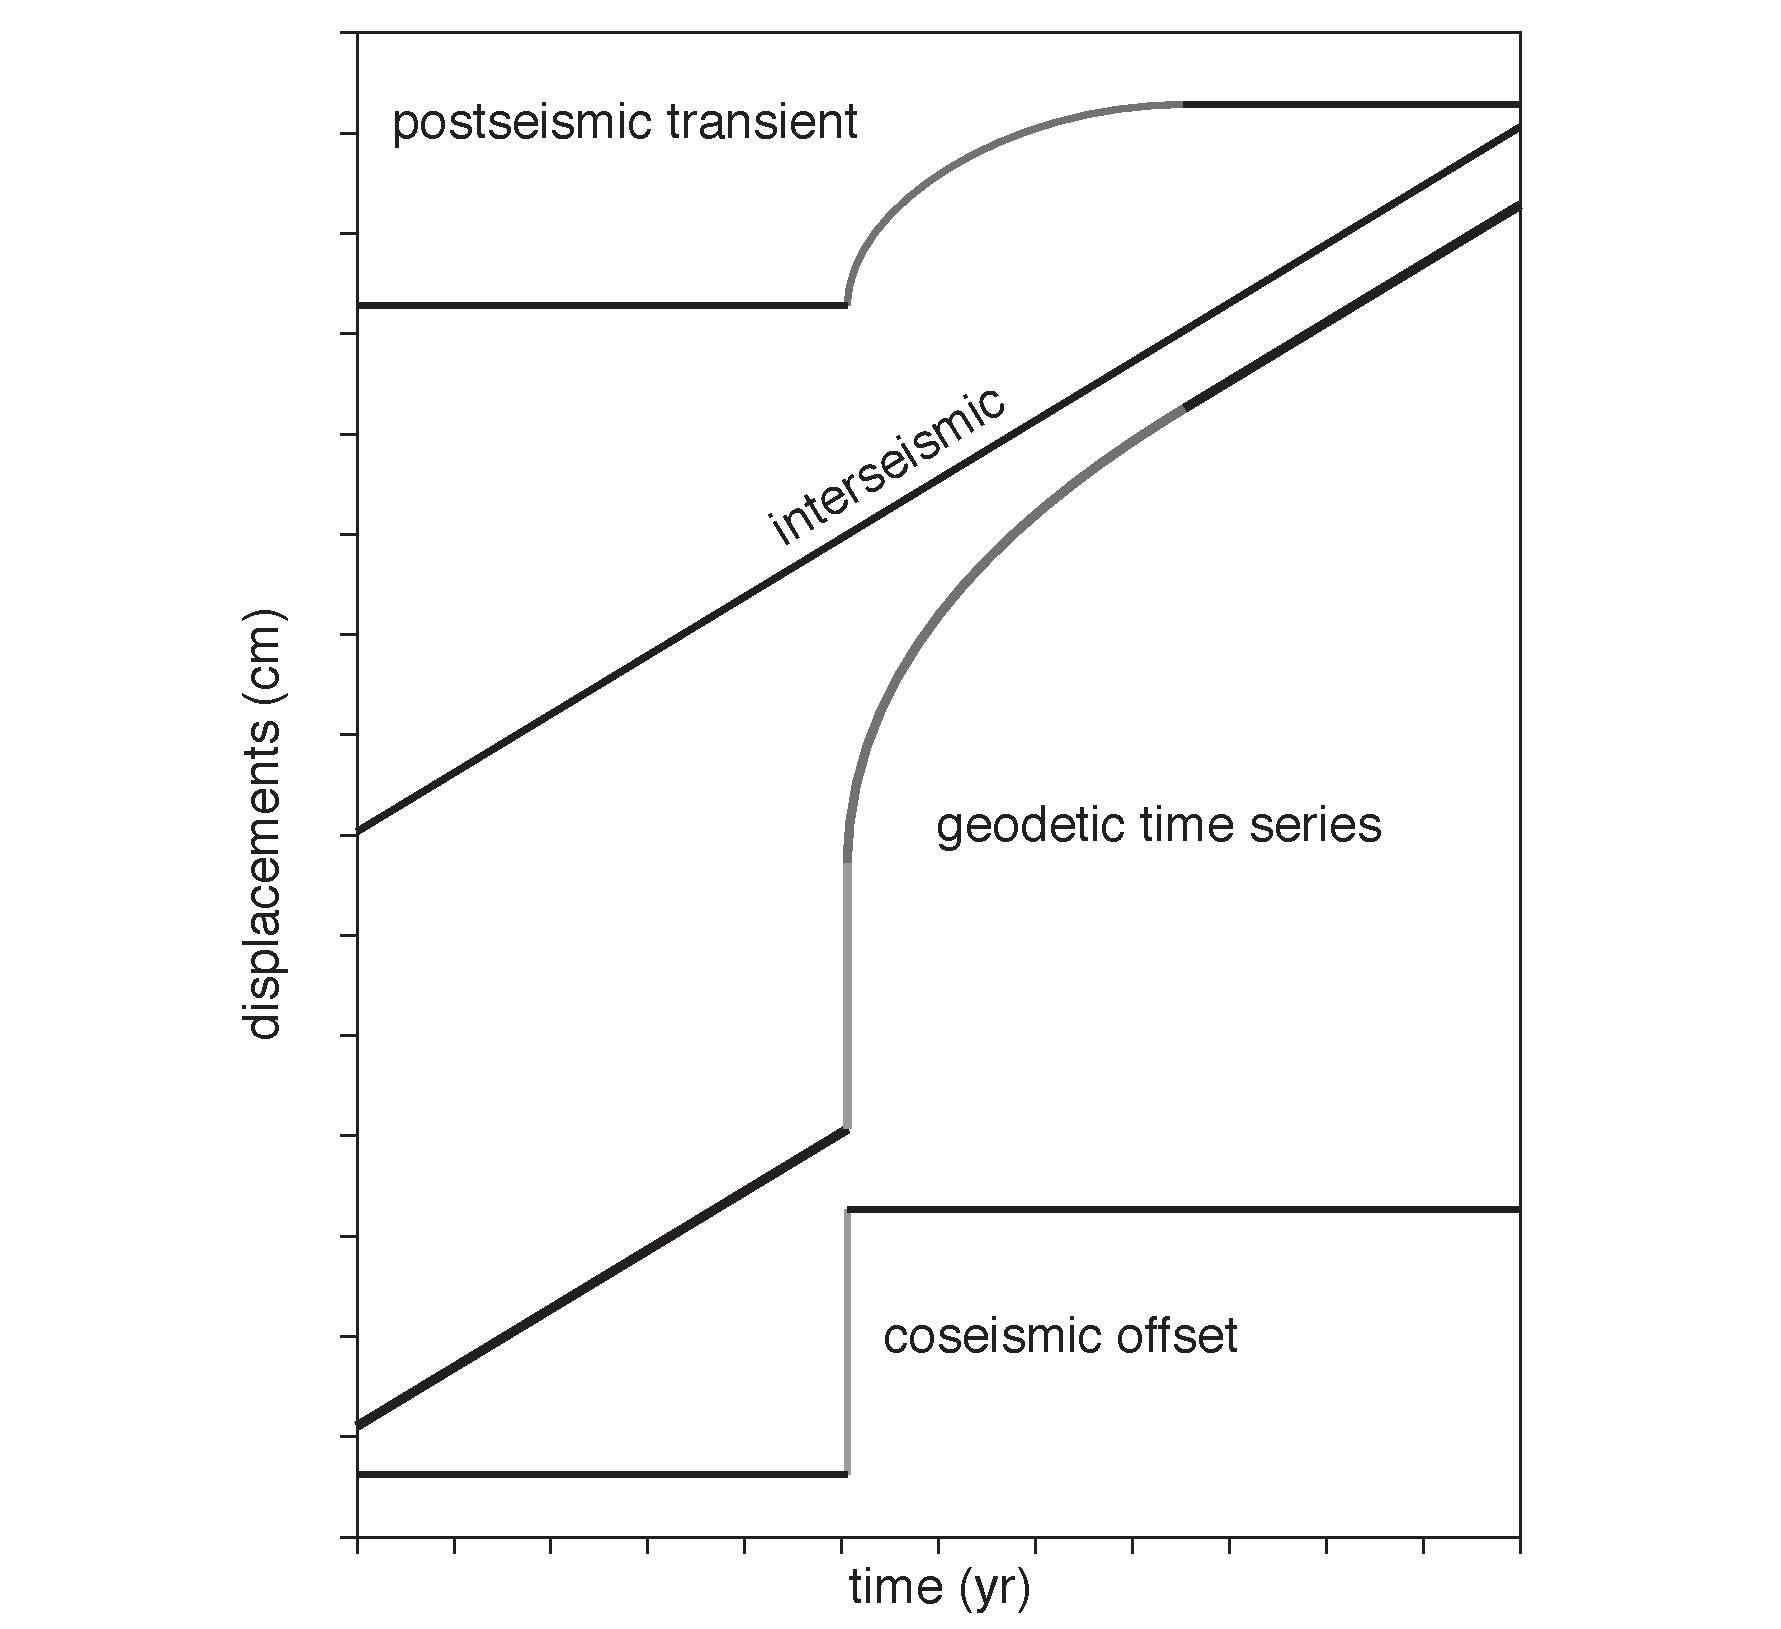
\includegraphics[width=1\textwidth]{seismic_cycle.pdf}
\end{center}
\end{figure}
\vspace{-0.5cm}
%
The \textbf{seismogenic zone} refers to the fault estate that produces large seismic ruptures. The rapid stress increase surrounding the earthquake causes a slip acceleration called \textbf{afterslip}, which can last several years. As the afterslip transient dissipates, the surface deformation in the rest of the interseismic period is due to fault \textbf{creep}, a steady slip with a velocity close to plate rate. This combination of events is thought to distribute slip on all parts of the fault, so that displacement is uniform over a full seismic cycle. \\
%
\begin{figure}[h]
\begin{center}
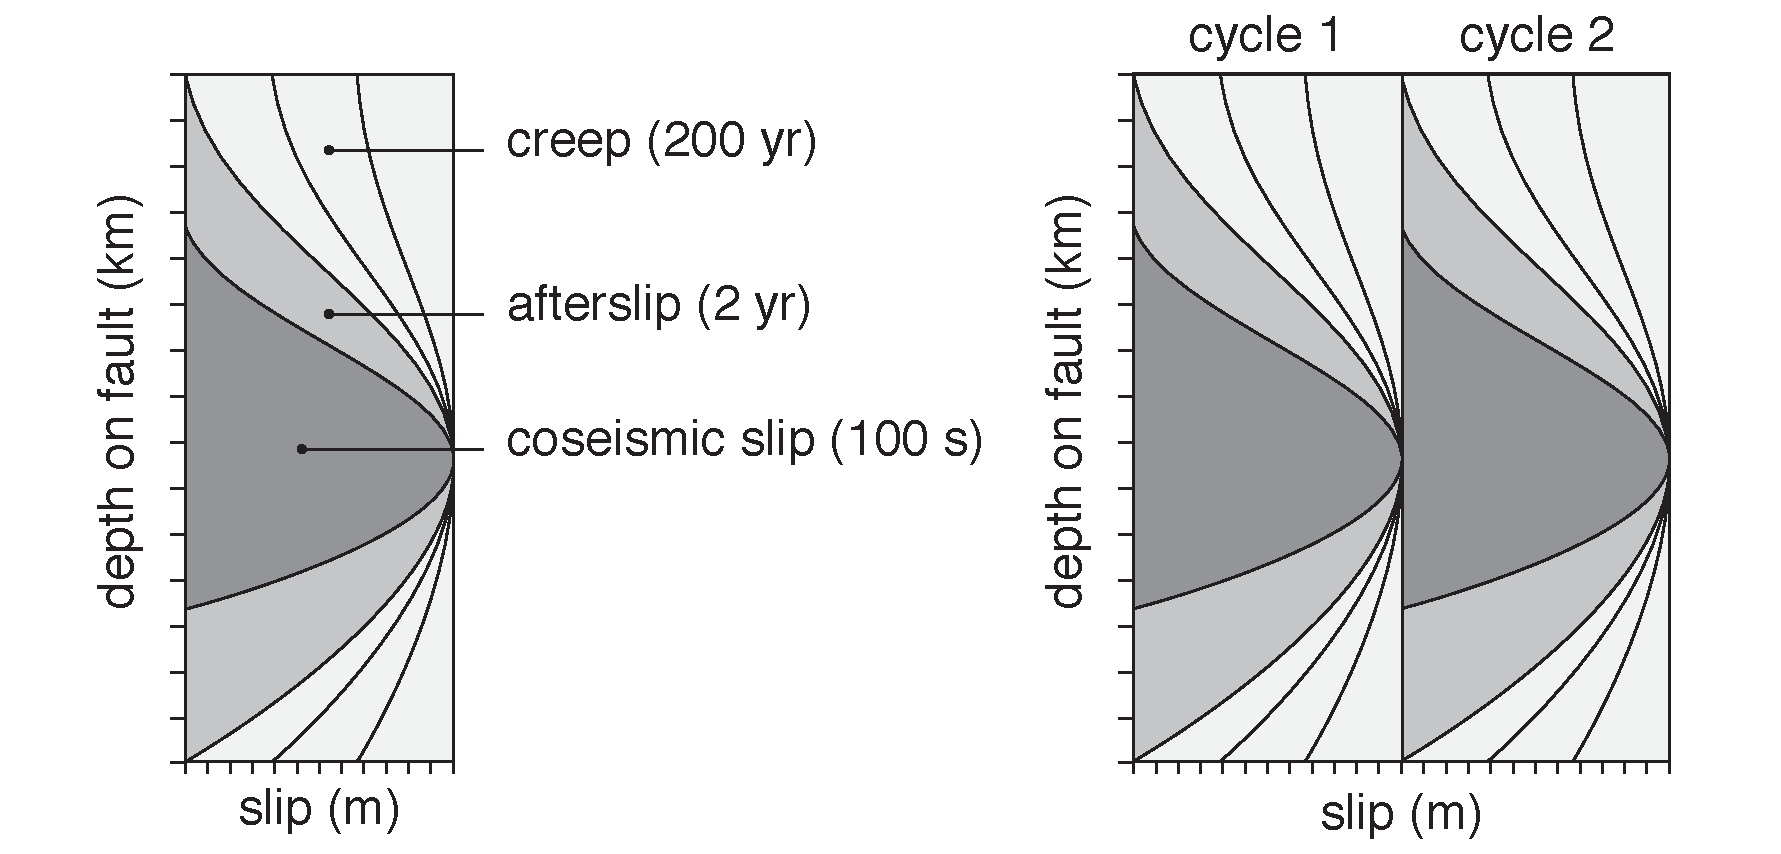
\includegraphics[width=1\textwidth]{seismic_cycle_fault.pdf}
\end{center}
\end{figure}
\vspace{-0.5cm}
%
\\
Many realistic aspects of faulting are ignored in this simple model, such as the effect of structure (fault geometry, branching and step-overs, heterogeneities in frictional properties), complexities arising spontaneously from the dynamics of fault slip (stress shadows), interactions with other faults (triggering mechanisms), and off-faults mechanics such as \textbf{viscoelastic flow}, \textbf{poroelastic} deformation, and \textbf{damage} evolution. In practice, it is rare to see seismic cycles repeating exactly like their predecessors. Faults can also slip suddenly during \textbf{slow-slip events}, which are impulsive in character, yet do not generate seismic waves like regular quakes. The duration of slow-slip ruptures can last several weeks.

\clearpage

\section{Velocity-jump experiments}

The earthquake cycle is thought to be an \textbf{elastic rebound} \citep{reid10}, whereby the strain accumulated during the interseismic period is released suddenly during earthquakes (or slow-slip events). This would require the frictional resistance to change over time. \\
%
\begin{figure}[h]
\begin{center}
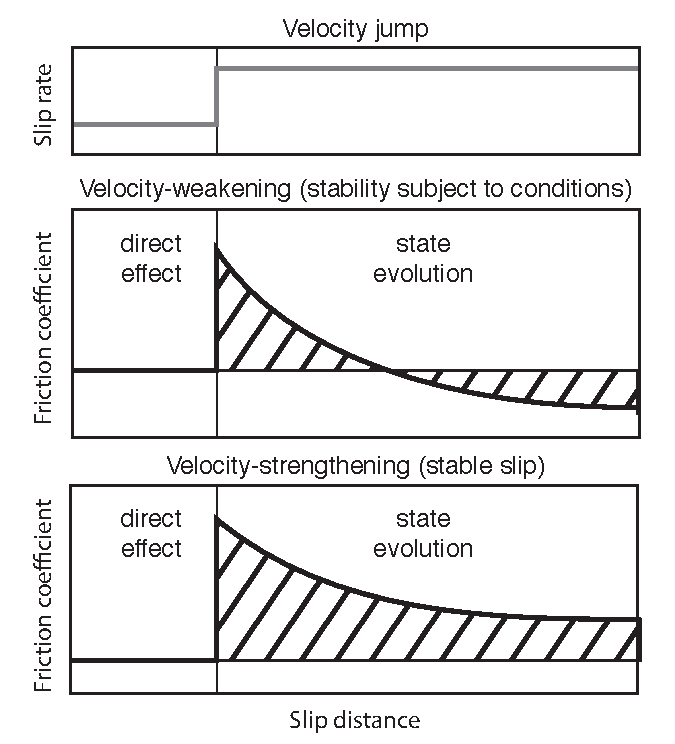
\includegraphics[width=0.7\textwidth]{velocity-strengthening-weakening.pdf}
\end{center}
\end{figure}
\vspace{-0.5cm}
%
\\
This is well illustrated in laboratory experiments that impose a velocity jump when sliding two rock samples past each other. The \textbf{velocity jump experiments} describe the evolution of the \textbf{frictional resistance} of the contact following the velocity increase. The velocity increase is always accompanied by an increased frictional resistance. The \textbf{direct effect} is the immediate resistance to increased slip velocity. This is a \textbf{strengthening} and \textbf{stabilizing} effect. Theoretical considerations indicate that faults would be unstable at all scales without it. The velocity jump is followed by a \textbf{state evolution} of the points of contact (microasperities) that is invariably weakening. If the final resistance is lower than before the velocity increase, the asperity contact follows a \textbf{velocity-weakening friction}. This is the basic ingredient for the generation of earthquakes and slow-slip events. If the final resistance is increased, this is referred to as \textbf{velocity-strengthening friction}. Velocity-strengthening friction is what is behind the creep and afterslip phenomena. \\
%
\\
Let's assume that the state evolution occurs over a characteristic distance $L$. Depending on the final amplitude of the coseismic slip $s$, the net friction change can be overall strengthening or weakening. We refer to this as the \textbf{conditional stability} of velocity-weakening asperities. Velocity weakening is a necessary, but not sufficient, condition for frictional instability. If slip $s$ is much greater than the characteristic distance $L$, then frictional instabilities can emerge. The system is called \textbf{conditionally unstable}. When earthquake slip is lower or of the order of $L$, the system is called \textbf{conditionally stable}. The final slip on a rupture depends on many aspects of the system, including the asperity size. It is therefore not possible to predict final slip based on friction properties alone.
%
\begin{figure}[h]
\begin{center}
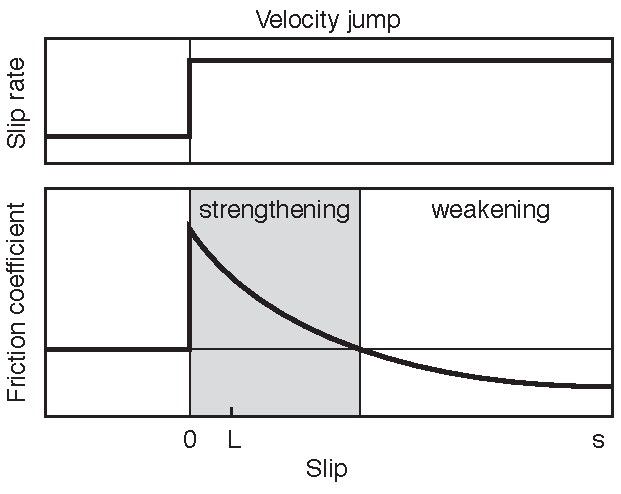
\includegraphics[width=0.7\textwidth]{conditional-stability.pdf}
\caption{Conditional stability of velocity-weakening asperities. If $s\gg L$, the asperity is conditionally unstable; if $s < L$, the asperity is conditionally stable.}
\end{center}
\end{figure}
\vspace{-0.5cm}
%


\clearpage

\section{Rate- and state-dependent friction}

Seismicity is inherently a stress relaxation process, whereby fault slip releases the forces that slowly built up during the preceding period of quiescence. The shear stress on faults accumulates gradually without much fault slip, at a pace controlled by the relative plate velocity and the degree of partitioning in a fault system. When the shear stress overcomes the \textbf{friction resistance} of the fault contact, it initiates a \textbf{slip instability}, which can result in radiation of seismic waves experienced as an earthquake.\\ 
%
\\
A key notion that allows us to understand the earthquake cycle is that the friction resistance of a fault is not constant. Friction resistance increases during the period of quiescence: this process is called \textbf{healing}; and it is \textbf{weakening} during slip. Studies of the strength evolution of fault surfaces was championed by \cite{dieterich72,dieterich78}, who showed that friction depends on the velocity of fault slip but also that it has a memory of the slip history. He determined that the strength of the fault recovers linearly with the logarithm of time. Dieterich coined the rate- and state-dependent friction model, whereby a state variable is used to represent the effect of healing and weakening. \\
%
\\
To represent the evolution of slip in a fault system, we use the framework of friction resistance, whereby the shear stress $\tau$ depends on the effective normal stress $\bar{\sigma}$ through the \textbf{consistency relation}
\begin{equation}\label{eqn:consistency}
\tau=\mu\,\bar{\sigma}=\mu\,(\sigma-p)
\end{equation}
where $p$ is the pore fluid pressure (both $\sigma$ and $p$ are assumed positive under compression). Why using the effective normal stress and not just the normal stress? The normal stress experienced by the micro-asperities can be reduced by pressurized fluids in the pore space of the fault zone. In general, the effective normal stress is $\sigma-\alpha p$, but we assume that the coupling between pore pressure and wall pressure is high in a fault zone and that the coefficient of effective stress $\alpha$ is one. Inclusion of the pore pressure in the consistency relation (\ref{eqn:consistency}) leads to all sorts of interesting phenomena, including strong weakening by thermal pressurization or by thermal activation of chemical decomposition~\citep[e.g.,][]{rice06a,sulem&famin09,noda&lapusta10}.\\
%
\\
In the context of rate- and state-dependent friction, the friction coefficient $\mu$ varies with the logarithm of the velocity of fault slip and with the logarithm of a state variable~\citep{dieterich78}
\begin{equation}\label{eqn:rateandstate}
\tau=\left[\mu_0+a\,\ln\left(\frac{V}{V_0}\right)+b\,\ln\left(\frac{\theta V_0}{L}\right)\right]\,\sigma
\end{equation}
while the state variable obeys its own evolution law. Here, for example, the aging law:
\begin{equation}\label{eqn:aginglaw}
\dot{\theta}=1-\frac{V\theta}{L}
\end{equation}
with the characteristic weakening distance $L$. The form of Eqs.~(\ref{eqn:rateandstate}) and (\ref{eqn:aginglaw}) is empirical, and we are still looking for its theoretical justification from the point of view of micro-mechanics. But the underlying idea is that a fault contact is rough at all scales and that micro-asperities must break to allow for fault slip and weakening. Chemical breakdown, fluidization, melting, phase transformation of fluids and rocks, fracturing, and pore fluid flow, are some of the processes that may contribute to the evolution of fault strength.\\
%
\\
The rate- and state-dependent friction formulation of~\cite{dieterich78} is only valid for slow slip regimes, $V\ll 0.1$\,m/s, before all the thermally activated processes and the seismic radiation become more dominant. It makes it an ideal \textbf{rheology} to model creep, afterslip, and slow-slip events. But it is also a starting point to model more sophisticated physical processes at high slip speed, granted that the set of governing equations is augmented accordingly. \\
%
%\begin{figure}[h]
%\begin{center}
%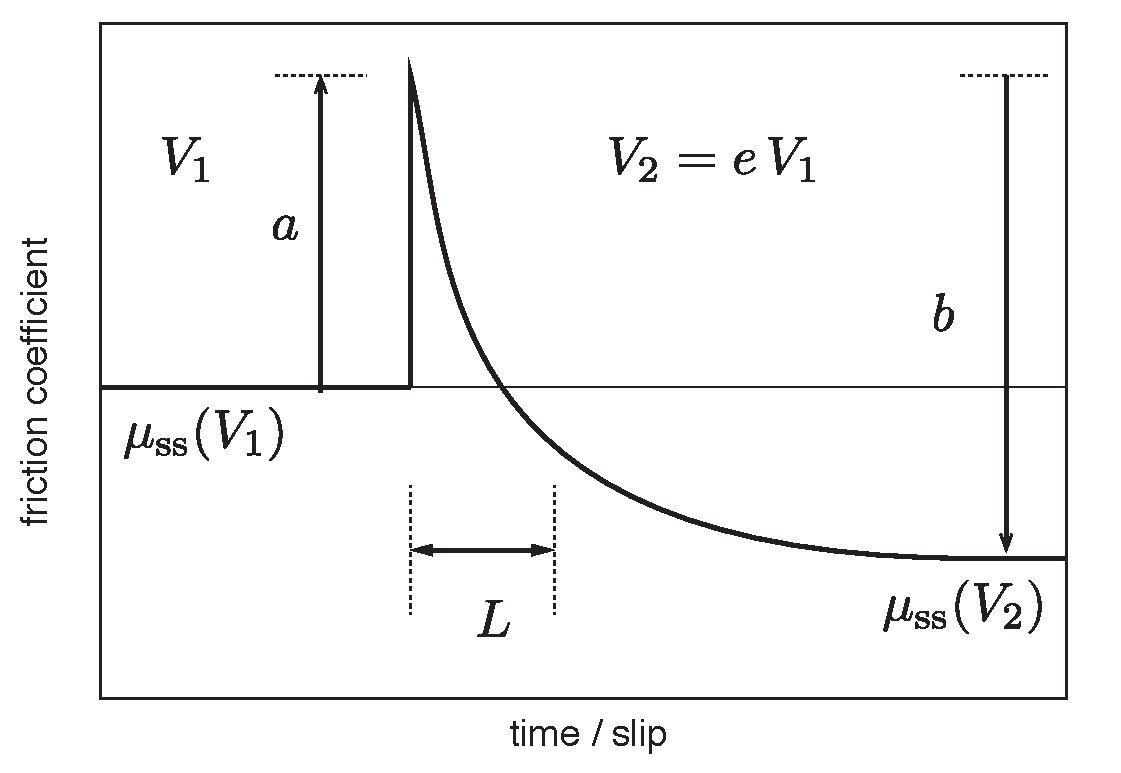
\includegraphics[width=0.7\textwidth]{friction-evolution.pdf}
%\end{center}
%\end{figure}
%
\\
To understand how the \textbf{constitutive equations} (\ref{eqn:rateandstate}) and (\ref{eqn:aginglaw}) work, let's look at the \textbf{steady state}. The steady state is an equilibrium state where all the forces are in balance and the dynamic variables stop evolving. In our case, it implies that there is a perfect equilibrium between the weakening and healing mechanisms and that $\dot{\theta}=0$. In this case, from Eq.~(\ref{eqn:aginglaw}), we get $\theta_\text{ss}=L/V$ and the steady-state friction is\\
%
\begin{equation}\label{eqn:steadystate}
\mu_\text{ss}=\mu_0+(a-b)\,\ln\left(\frac{V}{V_0}\right)
\end{equation}
%
\\
Despite the apparent complexity of Eqs.~(\ref{eqn:rateandstate}) and (\ref{eqn:aginglaw}), we can use Eq.~(\ref{eqn:steadystate}) to predict the long-term frictional resistance following a sudden increase of velocity, like at the passage of a seismic front. Eq.~(\ref{eqn:steadystate}) is also a good approximation to describe slip evolution in rate-strengthening areas at a limit when slip is much larger than $L$; this is the \textbf{rate-strengthening} approximation (the state evolution is ignored).\\
%
\begin{figure}[h]
\begin{center}
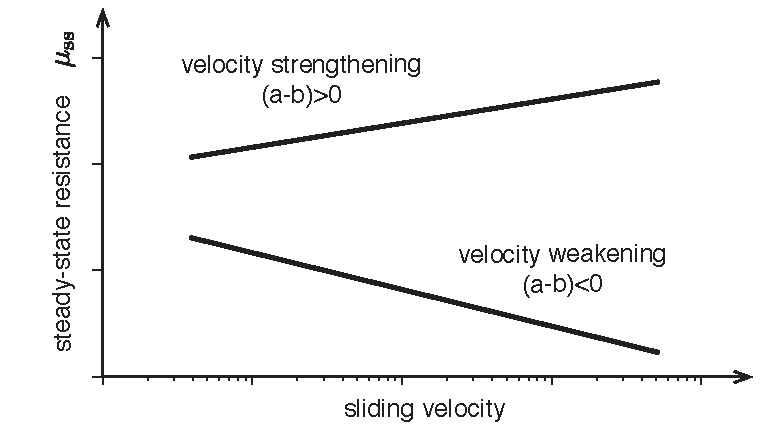
\includegraphics[width=0.9\textwidth]{rate-strengthening-approximation.pdf}
\end{center}
\vspace{-0.5cm}
\end{figure}
%
\\
Two regimes stand out, depending on the value of $(a-b)$. With $(a-b)>0$, high slip velocities imply more frictional resistance and this property is called \textbf{velocity-strengthening} friction. Velocity-strengthening areas of faults do not initiate seismic slip and hinder the propagation of seismic ruptures. When seismic asperities are surrounded by velocity-strengthening areas, we expect \textbf{afterslip} to occur around the rupture, in reaction to the sudden stress changes. With $(a-b)<0$, high slip velocities require less frictional resistance, and this \textbf{velocity-weakening} property is a necessary condition to generate frictional instabilities. Whether a velocity-weakening asperity will generate earthquakes depends on the details of the slip evolution, between one steady state to another. In loose terms, if this transition is short enough, the asperity is called \textbf{conditionally unstable}, or \textbf{seismogenic}. But if the transition takes longer, only slow-slip events may happen and the asperity is called \textbf{conditionally stable}. In this context, slow-slip events can be thought of as failed nucleations. Typical values for rate-and-state friction parameters are $\mu_0=0.6$, $a=10^{-2}$, $b=0.006$ for velocity-strengthening patches, $b=0.014$ for velocity-weakening patches.\\
\\
The factors that favor velocity-strengthening behavior in laboratory experiments are high temperatures ($>300^\circ$C), which leads to aseismic fault slip below certain depths~\citep{tse&rice86}; low effective normal stress, which leads to shallow velocity-strengthening layers and shallow slip deficit; certain types of rocks and fault gouge, for example the ones containing \textbf{clay minerals}; and the rock lithology (pulverized samples can be velocity strengthening while their intact fabric is velocity weakening).\\
\\
Many important effects occurring at high speed are ignored in the basic formulation of rate-and-state friction. These include the rapid shear heating, which is mostly weakening (flash weakening, lubrication)~\citep{tsutsumi&shimamoto97,ditoro+04,ditoro+06,ferri+10} and the associated pore-pressure changes~\citep{sibson73,bizzarri&cocco06a,noda&lapusta10,urata&kuge12}; the dilatancy (another state variable) and the associated pore pressure effects~\citep{segall&rice95,samuelson+11}; the quasi-static shear heating and associated changes, similar to a rate dependence; the dependence on the shear layer structure and its composition~\citep{santamarina&shin09,andrade+12}; the choice of the proper state-evolution law and the possibility of multiple state variables; the evolution of shear resistance in response to normal stress changes~\citep{linker&dieterich92}; and the (de-)mineralization of volatiles and associated heat and pore pressure effects~\citep{sulem&famin09}. Some of these effects can be added to the basic framework of rate-and-state friction.


\clearpage


\section{First-order estimates}

We can use the velocity-jump experiments to draw first-order estimates on important quantities that describe the seismic cycle. Seismic ruptures are not simple velocity jumps on faults, as a point on the fault experiences a range of slip velocities from the nucleation, to the propagation, to the termination of a slip event. But as the friction depends on the logarithm of the velocity, large changes in velocity have a similar effect - at least in terms of order of magnitudes. So we should indeed gain insight from velocity-jump experiments, but remember that it is not meant as a realistic earthquake source model.

\subsection{Stress drop}

From an initial steady-state situation at an initial stress, the direct effect associated with the velocity increase leads to a peak stress. As the asperity weakens, the fault reaches a new steady state and a new final stress. The \textbf{static stress drop} corresponds to the difference between the initial shear stress and the final shear stress. This is a static measure of the stress change, independent of the path followed in between. The \textbf{dynamic stress drop} is the peak-to-peak stress change, i.e., the difference between the peak stress and the final stress. \\
%
\begin{figure}[h]
\begin{center}
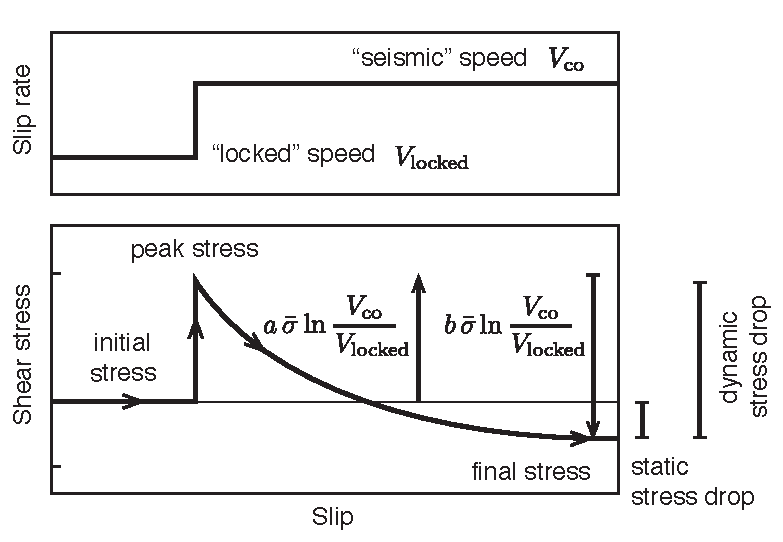
\includegraphics[width=0.8\textwidth]{rate-state-stress-drop-estimate.pdf}
\end{center}
\vspace{-0.5cm}
\end{figure}
%
\\
The static stress drop is an important measure of earthquake source, providing a proxy for average slip per unit area. This is also relevant to seismic hazards, connecting area of locked patches to magnitude estimates. In velocity-jump experiments, stress drop can be estimated from rate-and-state parameters and the effective confining pressure. Let's assume that the velocity jump occurs from a locked state, with a sliding velocity much lower than plate rate, say $V_\text{locked}=10^{-12}\,$m/s. (Here, we assume a loading rate of $V_\text{pl}=10^{-9}\,$m/s.) Suddenly, the fault is sliding at seismic speed, of the order of $V_\text{co}=1\,$m/s. The direct, strengthening, effect corresponds to a frictional resistance increase to \\
\begin{equation}
\tau_\text{peak}=\tau_\text{initial}+a\bar{\sigma}\ln\frac{V_\text{co}}{V_\text{locked}}~.
\end{equation}
After the state variable evolves, the frictional resistance reduces to
\begin{equation}
\tau_\text{final}=\tau_\text{initial}+a\bar{\sigma}\ln\frac{V_\text{co}}{V_\text{locked}}-b\bar{\sigma}\ln\frac{V_\text{co}}{V_\text{locked}}~.
\end{equation}
The dynamic stress is therefore
\begin{equation}
\Delta\tau_\text{dynamic}=b\bar{\sigma}\ln\frac{V_\text{co}}{V_\text{locked}}\simeq 10\,b\bar{\sigma}
\end{equation}
where we used estimates of the sliding velocities $\ln(V_\text{co}/V_\text{locked})\simeq 10$. The static stress drop follows
\begin{equation}
\boxed{\begin{aligned}
\Delta\tau_\text{static}\simeq 10~(b-a)\,\bar{\sigma}
\end{aligned}}
\end{equation}
The static stress drop depends on a combination of frictional properties and effective confining pressure. This formula is not directly applicable to earthquakes (in particular, the constant pre factor may be different), however, it does provide a way to understand how these physical parameters scale. For example, everything else being the same, you can predict how a change in pore pressure can affect stress drop.\\
\\
Assuming typical values for parameters $a$ and $b$, the ratio of dynamic to static stress drop is 
\begin{equation}
\frac{\Delta\tau_\text{dynamic}}{\Delta\tau_\text{static}}=\frac{b}{b-a}\simeq 3~.
\end{equation}

%\clearpage

\subsection{Slip}

\begin{table}
\centering
 \def\arraystretch{2}
\begin{tabular*}{0.85\columnwidth}{cccc}
 & Circular & Strike slip & $\quad$Dip slip \\
\hline
Strain drop $\Delta\epsilon$ & \parbox{1cm}{\begin{equation*} \frac{7\pi}{32}\frac{s}{R} \end{equation*}}  & \parbox{1cm}{\begin{equation*}\frac{1}{\pi}\frac{s}{W}\end{equation*}} & \parbox{1.5cm}{\begin{equation*}\frac{2}{\pi}\frac{\lambda+G}{\lambda+2G}\frac{s}{W}\end{equation*}}\\
Stress drop $\Delta\tau_\text{static}$ & \parbox{1cm}{\begin{equation*}\frac{7\pi}{16}G\frac{s}{R}\end{equation*}}  & \parbox{1cm}{\begin{equation*}\frac{2}{\pi}G\frac{s}{W}\end{equation*}} & \parbox{1.5cm}{\begin{equation*}\frac{4}{\pi}\frac{\lambda+G}{\lambda+2G}G\frac{s}{W}\end{equation*}}\\
\end{tabular*}
\vspace{0.5cm}
\caption{Stress drop for homogeneous slip $s$ on circular and rectangular dislocations~\citep{kanamori&anderson75}. Circular dislocations have a radius $R$. Rectangular dislocations have the (along-strike) length $L$ and (down-dip) width $W$, assuming $W<L$. $\lambda$ and $G$ are the Lam\'{e} parameters.}
\label{tbl:stress-strain-drops}
\end{table}

Analytic solution for stress and strain surrounding a circular dislocation~\citep{eshelby57} shows that the strain drop for a circular patch of radius $R$ and slip $s$ is
\begin{equation}
\Delta\epsilon=\frac{7\pi}{32}\frac{s}{R}
\end{equation}
The geometry of the asperity affects the strain drop and there are other estimate of strain and stress drops for rectangular dislocations. The coefficient in front of $s/R$ is often close to one so you will find it omitted sometimes. The stress drop in a surrounding medium with rigidity G is
\begin{equation}
\Delta\tau_\text{static}=\frac{7\pi}{16}G\frac{s}{R}
\end{equation}
This is a kinematic result based on the relationship $\Delta\tau_\text{static}=2G\Delta\epsilon$, independent of how you get there (rate-and-state or whatnot). Recall that for rate-and-state friction faults under a velocity jump, we have the static stress drop estimate $\Delta\tau_\text{static}\simeq 10~(b-a)\,\bar{\sigma}$. Equating both results, we get
\begin{equation}\label{eqn:slip}
\boxed{\begin{aligned}
s\simeq 5~\frac{(b-a)\,\bar{\sigma}}{G}R
\end{aligned}}
\end{equation}
This shows that the final slip in a circular asperity depends on both the frictional properties and the geometry. Again, this formula is not directly applicable to earthquakes, but it explains the relationship between final slip, friction properties, and the radius of the asperity. \\
\\
\textbf{Earthquakes slip scales with rupture dimension}: the longer the dimension, the larger the slip. This is because the boundary of the ruptures are pinned, so slip can be larger with greater distance to the no-slip boundary. This indicates that the critical dimension that controls slip and stress drop on non-circular asperities is the smallest of the along-strike and dip-dip patch dimensions. For long ruptures, the width (down-dip) of the asperity should be used to estimate slip and stress-drop. See Table~\ref{tbl:stress-strain-drops} for strain- and stress-drop estimates.

%\clearpage

\subsection{Recurrence time}
%
\begin{figure}[h]
\begin{center}
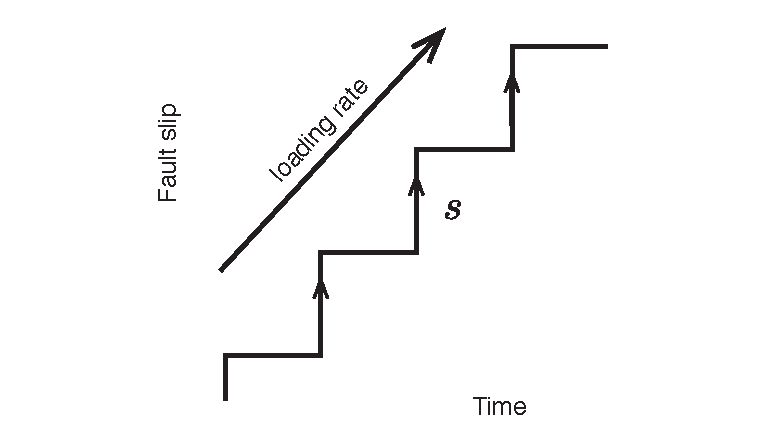
\includegraphics[width=0.8\textwidth]{recurrence-time.pdf}
\end{center}
\vspace{-0.5cm}
\end{figure}
%
The recurrence time of slip events must be compatible with the plate loading boundary condition. So we can write
\begin{equation}
\boxed{\begin{aligned}
T_r=\frac{s}{V_\text{pl}}\simeq 5\,\frac{(b-a)\,\bar{\sigma}}{G}\frac{R}{V_\text{pl}}
\end{aligned}}
\end{equation}
The model predicts a clock-work periodic system. This is not realistic. Faults produce earthquakes of variable stress drop, slip, and recurrence times. 


%\clearpage

\subsection{Stability}
Velocity-weakening asperity are conditionally stable or unstable depending on the amplitude of final slip. Assuming that the weakening occurs over a characteristic weakening distance $L$, if $s \gg L$, the asperity is conditionally unstable; if $s < L$, it is conditionally stable. We already have an estimate of slip based on asperity size and frictional properties (Eq. \ref{eqn:slip}). We can therefore write the stability condition based on the size of the asperity after defining the \textbf{critical nucleation size}
\begin{equation}
\boxed{\begin{aligned}
h^*=\frac{GL}{(b-a)\,\bar{\sigma}}
\end{aligned}}
\end{equation}
If $R\gg h^*$, the asperity is conditionally unstable; if $R<h^*$, it is conditionally stable. The stability of finite-size asperities depends on frictional properties and geometry. Small asperities are conditionally stable; large asperities are conditionally unstable.\\
%
\begin{figure}[h]
\begin{center}
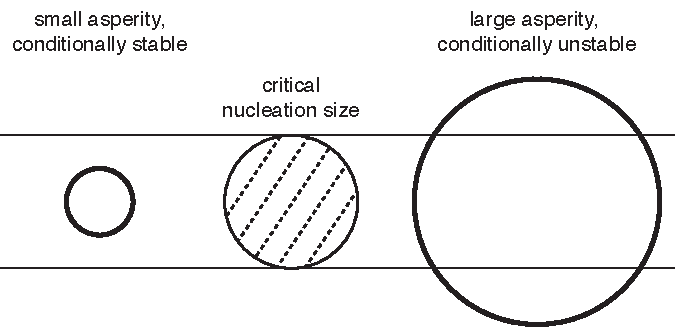
\includegraphics[width=0.9\textwidth]{nucleation-size-stability.pdf}
\end{center}
\vspace{-0.cm}
\end{figure}
%
\\
In practice, there is a spectrum of stability regimes for velocity-weakening asperities depending on the ratio $R/h^*$ going from creep, slow-slip events, \textbf{bilateral ruptures} and \textbf{unilateral ruptures}. The stability is affected by the geometry of the asperity. As corollary, the nucleation size can also be though of as the \textbf{minimum size} of earthquakes.\\
\\
The first-order estimates provide us with the means of explaining a particular seismo-tectonic context from frictional properties and geometry. Several pieces of information come available such as the recurrence times, or the stress drop, the magnitude, or the type of rupture (slow-slip events, unilateral or bilateral earthquakes). The characteristic weakening distance only affects the style of faulting through the critical nucleation size $h^*$. Changing the size of the asperity affects the slip in individual events and the recurrence time between events. The loading rate, frictional properties and dimension of the asperity must reconcile all these observations. This usually puts hard constraints on the distribution of $(a-b)$ on the fault, which defines the size of the asperity, and $(b-a)\bar{\sigma}$ and $L$ in the velocity-weakening region.

\clearpage

\section{The spring-slider system}

The mechanics of slip evolution is complex, but the earthquake cycle is often idealized by a spring-slider system~\citep{ruina83}. 
%
\begin{figure}[h]
\begin{center}
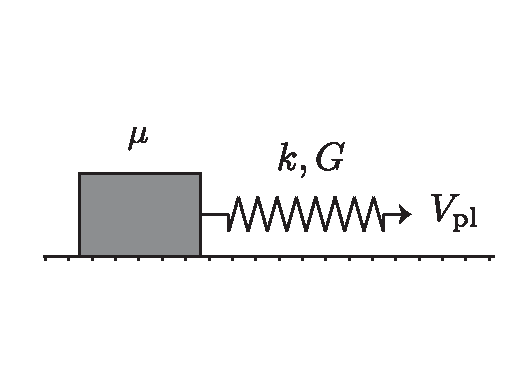
\includegraphics[width=0.5\textwidth]{spring-slider-setup.pdf}
\end{center}
\end{figure}
%
In this simple model, the tectonic forces are represented by a spring of stiffness $k$ that is loaded on one side at a constant stress rate $k\,V_\text{pl}$, where $V_\text{pl}$ is the plate rate, and resisted on the other side by a slider. The slider is thought to resist motion until the \textbf{yield stress} is reached. If the slider slips by a quantity $s$, it produces a stress decrease $k\,s$, called the \textbf{stress drop}. How does that relate to reality? \cite{eshelby57} showed that the stiffness of the spring-slider system can be related to the size of a seismic asperity through the relation
\begin{equation}\label{eqn:stiffness}
k=C\,\frac{G}{R}
\end{equation}
where $R$ is the linear dimension of the asperity (for example the radius for a circular crack or the half length for a square crack), $G$ is the shear modulus of the ambient rocks and $C$ is a constant close to $1$ that depends on the geometry~\citep{eshelby57,kanamori&anderson75,shearer99a,fi07a}. For a circular asperity, we have $C=7\pi/16$. Assuming that slip instabilities occur at a constant yield stress, Eq.~(\ref{eqn:stiffness}) predicts that the larger the asperity, the longer it can resist motion. \\
\\
But what is missing from this model? A lot. A single spring-slider system cannot represent the spatial distribution of fault slip, or the effect of the radiation of seismic waves or anything related to the interactions of several asperities or from different places with the same asperity, the so-called \textbf{long-range interactions}, to name a few examples. That being said, it produces helpful predictions that can help us understand the mechanics of more sophisticated settings, for example the work of~\cite{ruina83},~\cite{scholz98a} and~\cite{becker00}. Let's look at the balance of forces for the spring-slider system. Upon application of Newton's second law, and neglecting the acceleration, we get the equilibrium 
\begin{equation}\label{eqn:governingeq1}
\dot{\tau}+k\,V(\tau)=k\,V_\text{pl}
\end{equation}
Since $V$ and $\tau$ are related by the constitutive relation~(\ref{eqn:rateandstate})
\begin{equation}
V(\tau,\theta)=V_0\left(\frac{\theta V_0}{L}\right)^\frac{-b}{a}\exp\left(\frac{\tau-\mu_0\bar{\sigma}}{a\,\bar{\sigma}}\right)~,
\end{equation}
Eq.~(\ref{eqn:governingeq1}) represents an ordinary differential equation. More explicitly, we have a system of two coupled ordinary differential equations
\begin{equation}\label{eqn:governingeq2}
\left\{\begin{aligned}
&\dot{\tau}+k\,V(\tau,\theta)=k\,V_\text{pl}\\
&\dot{\theta}=1-V\theta/L
\end{aligned}\right.
\end{equation}
This looks horribly complicated, but if we write the vectors
\begin{equation*}
\begin{aligned}
\textbf{y}=\left(\begin{matrix}
s\\
\tau\\
\theta
\end{matrix}\right) & \qquad \quad\text{and} \qquad &
\dot{\textbf{y}}=\left(\begin{matrix}
V\\
\dot{\tau}\\
\dot{\theta}
\end{matrix}\right)
\end{aligned}
\end{equation*}
we find a system of the form $\dot{\textbf{y}}=f(t,\textbf{y})$, which is a canonical form that can be readily solved using numerical integration. Box~\ref{box:ss} shows how it can be solved in Matlab. 

\vspace{1cm}
\label{box:ss}
\begin{infobox}[\vspace{0.5cm}Box \ref{box:ss}. Modeling a single spring-slider system with Matlab]

In Matlab, there are a few functions that can solve a system of coupled ordinary differential equations. One of them is \textit{ode45}, where the 45 suffix stands for 4th-order/5th-order Runge-Kutta integration. The help of Matlab says
\begin{alltt}
>> help ode45
\textbf{ode45} Solve differential equations, medium order method.
 [T,Y]=ode45(FUN,TSPAN,Y0) with TSPAN=[T0 TF] integrates 
 the system of differential equations y' = f(t,y) from time 
 TO to TF with initial conditions Y0. ODEFUN is a function 
 handle. For a scalar T and a vector Y, ODEFUN(T,Y) must 
 return a column vector corresponding to f(t,y).
\end{alltt}
The algorithm implemented by \textit{ode45} can solve an ordinary differential equation solely equipped with a way to compute the time derivative of the dynamic variable numerically. The time steps are established automatically and optimally so as to satisfy a relative error criteria. A description of the algorithm can be found in the Numerical Recipes~\citep{press+92a}. \\
\\
To solve our system of equations in Matlab using \textit{ode45}, we can do the following. First, let's write a function called \textit{odefun.m} to describe the set of differential equations:

\begin{alltt}
{\color{blue}function} [yp] = odefun(~,y,ss)
V=2*ss.Vo*exp(...
 (y(2)-ss.mu0*ss.sigma-ss.b*ss.sigma*y(3))/(ss.a*ss.sigma));
yp=[V;ss.k*(ss.Vpl-V);(ss.Vo*exp(-y(3))-V)/ss.L];
{\color{blue}end}
\end{alltt}
%
You may have noticed that we used the logarithm of the state variable to integrate the aging law. As we use logarithms to evaluate fault strength, we need a numerical integration scheme that guarantees the positivity of the logarithmic argument. The state variable is a positive number, but it is flirting so close to zero (expected values are in the range [$10^{-12}$, $10^1$] seconds) that spurious numerical noise (think rounding errors) can make it ever so negative. In this case the logarithm of the state variable is a complex number and the calculation would become impossible. \\
\\
Then, we just have to set the friction parameters, solve the system numerically and plot the results. This can be done with the following script
\begin{alltt}
{\color{green}% static friction coefficient and normal stress}
ss.mu0=0.1;ss.sigma=50.0;
{\color{green}% stiffness}
ss.k=0.6;
{\color{green}% frictional parameters}
ss.a=1e-2;ss.b=ss.a+1.25e-3;
{\color{green}% characteristic weakening distance}
ss.L=0.1;
{\color{green}% plate velocity and reference slip rate}
ss.Vpl=1e-9;ss.Vo=1e-6;

{\color{green}% initialize the function handle with 
% set constitutive parameters}
yp=@(t,y) odefun(t,y,ss);

{\color{green}% solve the system}
opts=odeset('Refine',1,'RelTol',1e-14,'InitialStep',1e-7);
[t,Y]=ode45(yp,[0 3.1e10],...
   [ss.Vpl;ss.mu0*ss.sigma;0],opts);

{\color{green}% plot the state vector}
figure(1);clf;
subplot(3,1,1);cla;hold on
plot(t/3.1536e7,Y(:,1))
plot(t/3.1536e7,t*ss.Vpl,'r')
ylabel('slip (m)'), box on
subplot(3,1,2);cla
plot(t/3.1536e7,Y(:,2))
ylabel('stress (MPa)'), box on
subplot(3,1,3);cla
plot(t/3.1536e7,Y(:,3))
xlabel('time (yr)')
ylabel('ln (theta Vo / L)'), box on
\end{alltt}
With this set of parameters, the model spontaneously generates slow-slip events.

\end{infobox}
\vspace{1cm}


\section{Conditions for nucleation from linear stability analysis}

More insight about the behavior of the system of equations~(\ref{eqn:governingeq2}) comes from a powerful tool of applied mathematics called \textbf{linear stability analysis}. This technique allows you to predict the range of parameters that will lead to decaying or growing instabilities or oscillations upon perturbation of the system. \\
\\
The first step to analyzing the system is to describe a steady state when the system is loaded at the plate velocity. When the slider velocity, the state variable and the applied forces are all in equilibrium, we get $\dot{\theta}=0$, which implies a perfect balance between healing and weakening. From the aging law~(\ref{eqn:aginglaw}), this gives
\begin{equation} 
\theta^\text{ss}=\frac{L}{V}
\end{equation}
and the steady-state strength evolution
\begin{equation}
\dot{\tau}^\text{ss}=k\,(V_\text{pl}-V)
\end{equation}
We now define new dynamic variables that are deviations from the steady-state values (deviation from equilibrium)
\begin{equation}
\begin{aligned}
\tau^*=\tau-\tau^\text{ss}(V_\text{pl}); & \qquad & \theta^*=\theta-\theta^\text{ss}(V_\text{pl}); & \quad & V^*=V-V_\text{pl}+\dot{\tau}^\text{ss}/k
\end{aligned}
\end{equation}
and we linearize the system of equations~(\ref{eqn:aginglaw}) around the steady-state value:
\begin{equation}\label{eqn:linearized-system}
\begin{aligned}
\dot{\tau}^*&=F_{\!,\theta}\,\dot{\theta}^*+F_{\!,V}\,\dot{V}^*=-kV^*\\
\dot{\theta}^*&=G_{\!,\theta}\,\theta^*+G_{\!,V}\,V^*
\end{aligned}
\end{equation}
where the $F_{\!,\theta}$, $F_{\!,V}$, $G_{\!,\theta}$ and $G_{\!,V}$ are the coefficients of variation of the strength and the state variable around the steady state:
\begin{equation}
\begin{aligned}
F_{\!,\theta}&=\left.\frac{\partial\tau(V,\theta)}{\partial\theta}\right|_{\theta^\text{ss}}=b\bar{\sigma}\frac{V}{L}\\
F_{\!,V}&=\left.\frac{\partial\tau(V,\theta)}{\partial V}\right|_{\theta^\text{ss}}=\frac{a\bar{\sigma}}{V}
\end{aligned}
\end{equation}
and
\begin{equation}
\begin{aligned}
G_{\!,\theta}&=\left.\frac{\partial\dot{\theta}(V,\theta)}{\partial\theta}\right|_{\theta^\text{ss}}=-\frac{V}{L}\\
G_{\!,V}&=\left.\frac{\partial\dot{\theta}(V,\theta)}{\partial V}\right|_{\theta^\text{ss}}=-\frac{1}{V}
\end{aligned}
\end{equation}
%
We now look for a solution of the linearized system~(\ref{eqn:linearized-system}) of the form
\begin{equation}
\begin{aligned}
\tau^*=\text{Re}[A_1\,e^{st}]; & \qquad & \theta^*=\text{Re}[A_2\,e^{st}]
\end{aligned}
\end{equation}
where $\text{Re}[~]$ denotes the real part of its argument, $A_1$ and $A_2$ are constants, and $s$ is a constant to be determined. A positive real part of $s$ corresponds to a growing instability. Purely complex values of $s$ correspond to oscillatory modes and negative real parts of $s$ correspond to decaying instabilities. \\
\\
Let's solve for $s$! From the second equation of~(\ref{eqn:linearized-system}) we get 
\begin{equation}
\begin{aligned}
V^*&=\frac{A_2}{G_{\!,V}}\left(s-G_{\!,\theta}\right)\,e^{st}\\
\dot{V}^*&=\frac{A_2}{G_{\!,V}}\left(s^2-G_{\!,\theta}\,s\right)\,e^{st}
\end{aligned}
\end{equation}
which we can use to eliminate $V^*$ and $\dot{V}^*$ from the first equation, to obtain the following quadratic equation for $s$ in canonical form:
\begin{equation}
s^2+\frac{G_{\!,V}\,F_{\!,\theta}-F_{\!,V}G_{\!,\theta}+k}{F_{\!,V}}\,s-k\frac{G_{\!,\theta}}{F_{\!,V}}=0\\
\end{equation}
The solution is given by
\begin{equation}
\begin{aligned}
s&=\frac{-T\pm\sqrt{T^2-4D}}{2}\\
\end{aligned}
\end{equation}
with
\begin{equation}
\begin{aligned}
T&=\frac{-1}{a\bar{\sigma}}\frac{V}{L}\big[(b-a)\bar{\sigma}-kL\big]\\
D&=\frac{1}{a\bar{\sigma}}\frac{V}{L}\,kV
\end{aligned}
\end{equation}
As $D$ is positive, $s$ has a positive real part if and only if
\begin{equation}
k<\frac{(b-a)\bar{\sigma}}{L}
\end{equation}
This means that the spring-slider system will only generate slip instabilities if both $(b-a)>0$ and the spring stiffness is lower than a critical value. This makes sense, because as a limit, for an infinitely stiff spring, the slider is forced to move at plate velocity. The stiffness has to be low enough to allow for the spring to load elastic energy and for the slider to release it in sudden motions. This behavior is called \textbf{stick-slip} motion.\\
\\
How does that relate to real life again? Remember that through Eq.~(\ref{eqn:stiffness}) we can relate the equivalent stiffness to the size of an asperity ($k=G/R$). This implies that given a set of dynamic friction properties and an effective confining pressure, only asperities with a dimension greater than the \textbf{critical nucleation size}
%
\begin{equation}
\boxed{h^*=\frac{GL}{(b-a)\,\bar{\sigma}}}
\end{equation}
%
can generate frictional instabilities. If both $(b-a)>0$ and $R>h^*$, then the system is called conditionally unstable. If $(b-a)>0$ but $R<h^*$, the system is called conditionally stable.\\
\\
At the point of \textbf{neutral stability}, where $k=(b-a)\bar{\sigma}/L$, $s$ is purely imaginary and the stress evolution is oscillatory. 
\begin{equation}
\begin{aligned}
\tau^*(t)=A_1\,\cos\left(2\pi\,\frac{t}{T}\right)
\end{aligned}
\end{equation}
with a period
\begin{equation}
T=2\pi\,\frac{L}{V}\sqrt{\frac{a}{b-a}}=2\pi \,R\,\frac{(b-a)\bar{\sigma}}{G V}\sqrt{\frac{a}{b-a}}
\end{equation}
These results were brought to light by~\cite{ruina80,ruina83}, who also predicted for the first time the possibility of \textbf{creep waves}. \cite{ruina80} writes "The oscillations in the spring-block model [can] become propagating creep waves. Whether or not such waves are seen or can be seen in nature is not yet known". Slow-slip events have finally been observed some twenty years later~\citep{rogers&dragert03,schwartz&rokosky07,ito+07,vergnolle+10} in all ocean-continent subduction zones except in Sumatra/Java. They usually occur below the seismogenic zone in the transition depths between velocity-weakening and velocity strengthening properties. However, slow-slip events have many characteristics that may not all be explained by neutral stability~\citep{rubin08,rubin11}.

\section{Energy}

During a slip instability, the available energy is dissipated by the frictional heating and the fracture processes, and radiated away by seismic waves. There is a large spectrum of slip instabilities, going from slow slip events, to slow earthquakes to normal earthquakes and super-shear earthquakes.

\section{Radiation damping}

We need to be able to model earthquakes in the context of boundary integral method. The key to doing this is radiation damping. This takes care of energy radiation by energy dissipation. This is cool. 

Second Matlab box.

\clearpage




% % % % % % % % % % % % % % % % % % % % % % % % % % % % % % % % % % % % % % % % % % % % %
% % % % % % % % % % % % % % % % % % % % % % % % % % % % % % % % % % % % % % % % % % % % %
% % % % % % % % % % % % % % % % % % % % % % % % % % % % % % % % % % % % % % % % % % % % %
% % % % % % % % % % % % % % % % % % % % % % % % % % % % % % % % % % % % % % % % % % % % %


\chapter{Earthquake cycle and geometry}

\clearpage

\section{Conservation of motion}

As much as the physics of faulting exerts a first-order control on all aspects of earthquake and slow-slip event generation, geometry plays a dominant role. In fact, the geometry of fault systems controls some of the most important aspects of the earthquake cycle, such as \textbf{segmentation} and \textbf{slip partitioning}. The structural control of the earthquake cycle is evident from the concentration of earthquakes in the continental crust, both in intra-plate and subduction zone contexts.\\
%
\begin{figure}[h]
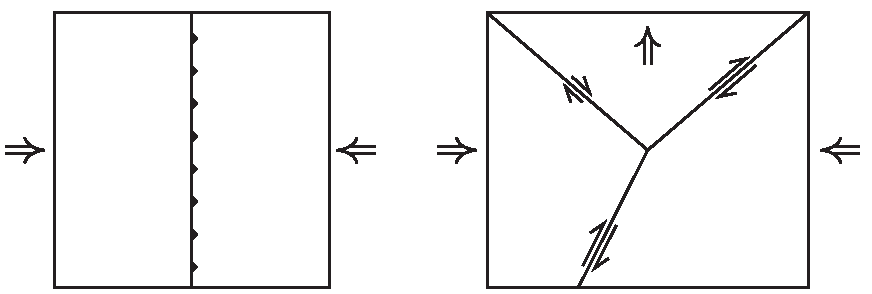
\includegraphics[width=\columnwidth]{convergence.pdf}
\end{figure}
%
\\
To understand the fundamental role of geometry, we need to think about the \textbf{conservation of motion} around a plate boundary. The relative velocity across a plate boundary is dictated by the motion of \textbf{tectonic plates}, which can be thought of a far-field \textbf{kinematic boundary conditions} that dictate the long-term kinematics of the plate boundary (Dirichlet boundary condition). The relative motion can be accommodated by various different configurations of systems of faults. For example the same plate convergence can be accommodated by a single subduction zone, or by a a system of strike-slip faults. The difference is that for a subduction zone, material escapes out of the plane while for a strike-slip system material escape in the plane. But both systems represents two different ways to materialise conservation of motion in the horizontal direction. \\
%
\begin{figure}[h]
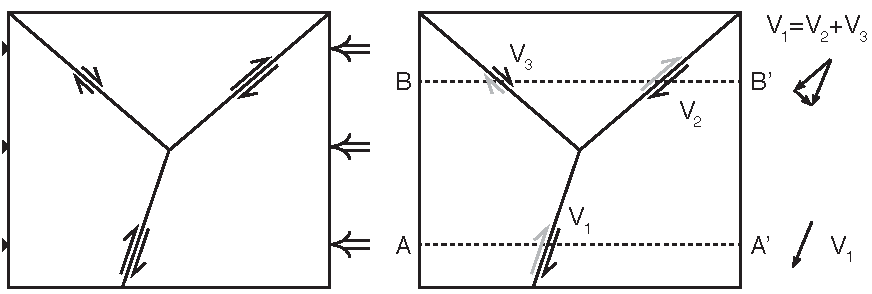
\includegraphics[width=\columnwidth]{conservation-depth.pdf}
\end{figure}
%
\\
To understand the implications of conservation of motion, let's consider a simple system where two plates converge towards each other. We are going to stipulate that the convergence of the plates is uniform at depth. This means that in the far field, particles at the same depth across the plate boundary converge at the same speed. Next, we suppose that the convergence is supported by faults, which take all of the deformation. In this case, the sum of the slip vector at all faults found at a given depth should add up to the same far-field relative velocity vector.\\
\\
Let us consider the case of a \textbf{ramp-d\'{e}collement} configuration under uniform convergence. The slip vectors must be parallel to the fault. To satisfy the far-field boundary conditions the projection of the slip vectors on the horizontal plane must be the same on the ramp and on the d\'{e}collement. If not, the top of the plate would move at a different convergence rate than the bottom of the plate. But this implies that the absolute slip velocities on the two faults are different in the dip direction: there is a \textbf{residual velocity} in the system. Particles belonging to the same upper block move at different velocities, leading to unbounded accumulation of stress. As rocks break above a \textbf{yield stress}, the fault system will ultimately be augmented with a new fault or a new fault system.\\
%
\begin{figure}[h]
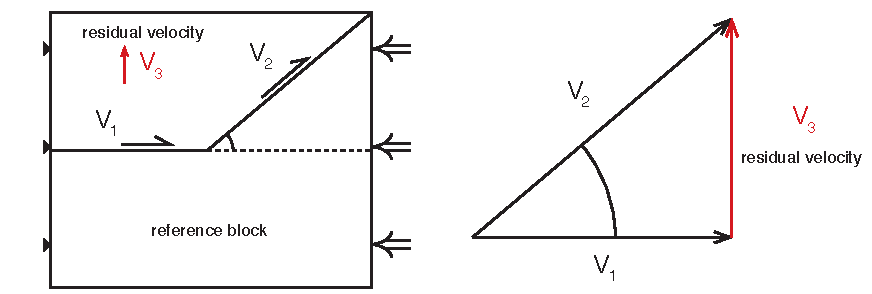
\includegraphics[width=\columnwidth]{ramp-decollement-residual.pdf}
\end{figure}
%
\\
A system of faults is said to \textbf{conserve motion} if the net residual velocity is null. A system of three fault segments can conserve motion, but other geometries are possible. An \textbf{odograph} conveniently portrays the kinematics of the system. To avoid the unbounded stress accumulation in the system, the slip velocity vectors must form a closed loop. The secondary fault segment that closes the velocity loop is called a \textbf{kink fault}. As the slip velocity must be parallel to the fault, the odograph predicts the slip velocity (normal or thrust motion) and the \textbf{orientation} of the kink fault. Two faults can impersonate the velocity vector, one pointing towards the surface, and another pointing towards depth (dashed line above). The fault pointing towards the free surface should be retained as it is the one requiring the least mechanical work and therefore this choice minimises the energy of the system.\\
%
\begin{figure}
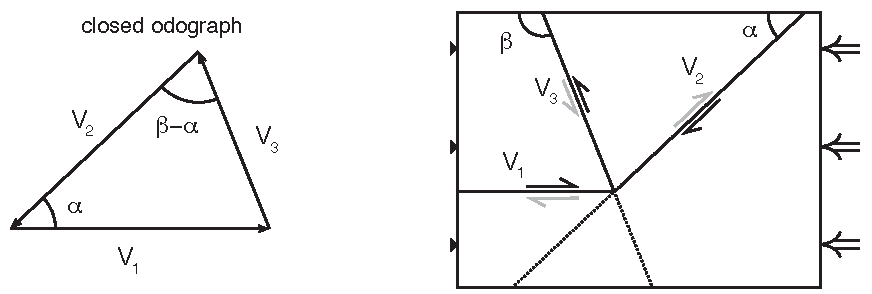
\includegraphics[width=\columnwidth]{ramp-decollement-odograph.pdf}
\end{figure}
%
\\
The most important implication of the conversation of motion is that \textbf{geometry controls the long-term slip velocity of faults}. If we change the relative angles between these faults, the relative velocities must change accordingly. Application of the \textbf{law of cosines}, from the Persian mathematician and astronomer Al-Kashi, implies the following relationships between slip velocity and relative angles\\
\begin{equation}
\boxed{\begin{aligned}
\hspace{0.5cm}\frac{V_2}{V_1}&=\frac{\sin\beta}{\sin(\beta-\alpha)}\hspace{0.5cm}\\
\frac{V_3}{V_1}&=\frac{\sin\alpha}{\sin(\beta-\alpha)}
\end{aligned}}
\end{equation}
%
The laws of conservation of motion are fundamental to plate tectonics and they can be applied both in map view and cross section. The relative convergence between plates can be distributed among an arbitrary number of faults. The \textbf{flower structure} is a system of decreasing complexity with depth, where all branches of faults at shallow depth merge into a single tree trunk, all the while conserving motion at every depth level.\\
%
\begin{figure}
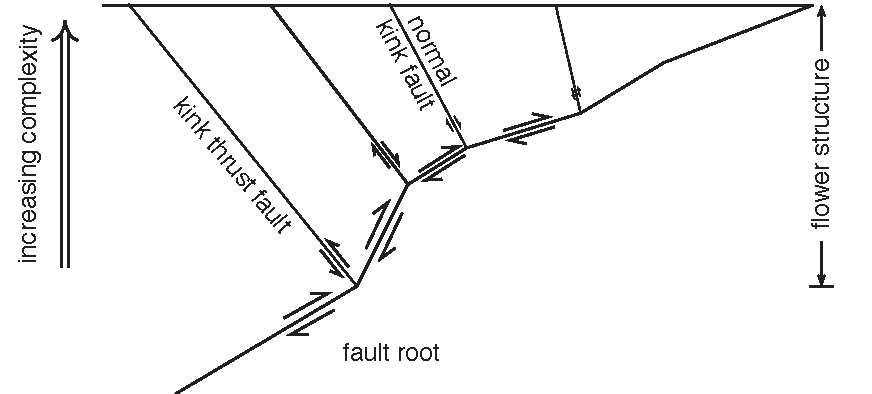
\includegraphics[width=\columnwidth]{flower-structure.pdf}
\end{figure}
%
\\
Another aspect about junction of faults is whether a configuration is stable or not. This is an important aspect of the long-term evolution of plate boundaries. A fault system is \textbf{unstable} if motion of the fault inherently disrupt the geometry of the system, like triple junctions of strike-slip faults. Unstable systems can be found everywhere on Earth in map view and cross section. The stability of the system is important to consider at geological time scales (say a few million years), but it is less important for time scales relevant for the earthquake cycle (say a few thousand years or ten recurrence times of large earthquakes). Triple functions of strike-slip faults (in map view) or dip-slip faults (in cross section) are unstable. More sophisticated descriptions of motion in balanced cross sections provide a stable system \citep{suppe81}.

\clearpage

\section{Slip partitioning}

The

\begin{sidewaysfigure}[p]
\captionwidth{0.9\linewidth}
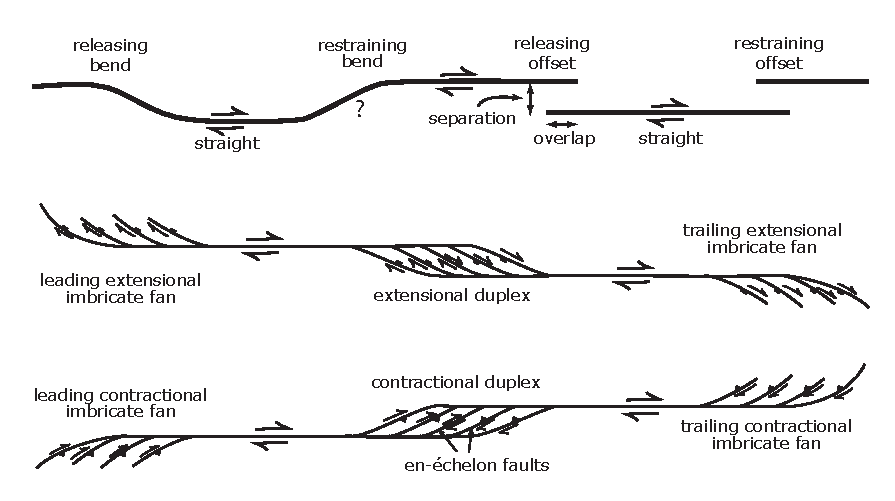
\includegraphics[width=\textwidth]{woodcock+fisher86fig1.pdf}
\caption{Nomenclature describing strike-slip fault systems from \cite{woodcock&fischer86}.}
\label{fig:fluidity}
\end{sidewaysfigure}


\clearpage

% % % % % % % % % % % % % % % % % % % % % % % % % % % % % % % % % % % % % % % % % % % % %
% % % % % % % % % % % % % % % % % % % % % % % % % % % % % % % % % % % % % % % % % % % % %
% % % % % % % % % % % % % % % % % % % % % % % % % % % % % % % % % % % % % % % % % % % % %
% % % % % % % % % % % % % % % % % % % % % % % % % % % % % % % % % % % % % % % % % % % % %

\chapter{Postseismic viscoelastic relaxation}

\clearpage



\section{Viscoelasticity}

At high temperatures, or over long periods, the Earth's rocks behave like \textbf{viscous fluids}. This is most clearly evidenced by magmatic flow, where hot lava can travel long distances like fluids do, but quickly changes into a solid rock as the material cools down. The fluid properties of rocks are critical to allow deep \textbf{mantle convection} and plate tectonics. A typical value of the \textbf{viscosity} of rocks is in the range $\eta=10^{17}-10^{23}\,$Pa\,s and with greater viscosities rocks are considered elastic or brittle. The wide range of viscosities is explained by the temperature dependence of viscosity through an \textbf{Arrhenius law}: We say that the viscosity of rocks is \textbf{thermally activated}. As temperatures overall increase with depth, in general viscous flow occurs deep into the lower crust (or the upper mantle) below a \textbf{rigid lid}. As viscous flow of mantle rocks is measured through the elastic deformation of the top lid, both the viscous and elastic properties of rocks need to be considered together. We refer to this type of material as \textbf{viscoelastic}. \\
\\
Viscoelastic materials are elastic at short time scales and viscous at long time scales. Elastic materials deform instantaneously with applied load, so that \textbf{Hooke's law} $\epsilon=\tau/G$, where $G$ is the rigidity, $\tau$ is the shear stress and $\epsilon$ is the strain, always applies. Viscous material are such that the rate of deformation scales with shear stress. In its simplest form, it can be written as a \textbf{Maxwell rheology}
\begin{equation}
\dot{\epsilon}^i=\frac{\tau}{\eta}
\end{equation}
where $\epsilon^i$ is the total \textbf{inelastic strain}. The fundamental difference between elastic and viscous flow is that the viscous deformation represents \textbf{irreversible strain}, i.e., the material does not return to its original configuration if the applied load is removed. The energy is absorbed by the system and used for permanent changes in the microstructure. When the viscosity $\eta$ is constant (not stress dependent), this corresponds to a \textbf{Newtonian fluid}. In this case the stress/strain-rate constitutive relationship is linear; this is referred to as a linear fluid, a linear viscosity, or a \textbf{linear rheology}. For viscoelastic materials, we have both elastic and viscous behaviors, and the elastic and inelastic strain components add up. The total strain can then be written in the form
\begin{equation}
\dot{\epsilon}=\frac{\dot{\tau}}{G}+\frac{\tau}{\eta}
\end{equation}
If the viscosity depends on stress, we refer to the material as a \textbf{power-law}, or as a \textbf{non-Newtonian fluid}. Regardless of the type of rheology, the \textbf{effective viscosity} can be defined as
\begin{equation}
\eta_\text{effective}=\frac{\tau}{\dot{\epsilon}}
\end{equation}
the ratio of stress to strain rate. Oftentimes, only the effective viscosity can be inferred from field measurements so in this case, its meaning in terms of micromechanics is subject to interpretation. Constraining effective viscosity from geodetic observations can be useful to explain quasi-static stress transfers and postseismic deformation, but the different stress perturbations to the crust and mantle will likely give rise to different effective viscosities, so in that sense, effective viscosity does not have predictive power. \\
\\
There are several methods to infer the mantle viscosity, depending on length and time scales. Typically, long phenomena constrain deep properties, and short phenomena are sensitive to a shallower structure. The mantle viscosity can be inferred from the dynamics of the hydrosphere. For example, the \textbf{postglacial rebound} following periods of glaciation offers a way to constrain viscosity deep into the mantle. Below Fennoscandia and Greenland the rapid melting of kilometer-thick ice sheets at the onset of the current warm period 20,000 years ago suddenly unloaded the Earth's surface and triggered a viscoelastic readjustment that still persists today. The evolution of paleo-shorelines can be related to the time-dependent viscoelastic rebound. Rapid variations in water storage due to \textbf{lake refills and drainage}, both natural and anthropogenic, also create a load on the crust (negative or positive) that is followed by a transient displacement.  Another way to infer deep mantle viscosity is to exploit the periodic surface \textbf{loading from the monsoon}. The effective rigidity, $G^\text{effective}=\tau/\epsilon$, of viscoelastic materials is frequency dependent, so the amplitude of the deformation and its phase delay can be related to the mantle viscosity. The viscosity of lower-crustal rocks can also be inferred from \textbf{paleo-piezometry} of exhumed rocks, as the grain size of quartz crystals can be related to the ambient stress (viscosity and stress are related by the strain rate). Another method to probe into the \textbf{inelastic properties} of the lower crust and the upper mantle is using the postseismic relaxation triggered by large earthquakes. Long after seismic waves attenuated away and the ground stopped shaking, a \textbf{quasi-static deformation} of viscoelastic rocks still persists. Viscoelastic relaxation following large earthquakes endures for years and decades, and can be measured geodetically. Here, we are interested in the modeling of \textbf{earthquake cycles} including the effect \textbf{off-fault deformation} and postseismic \textbf{viscoelastic relaxation}.


\section{Strain localization}

The deformation in the lithosphere exhibits various degrees of \textbf{strain localization}. Faults represent the ultimate localization of deformation and the fault zone is a region of increased \textbf{damage}. The \textbf{fault core} is formed by \textbf{cataclastic rocks} formed by fracturing during faulting. Below the seismogenic zone, near the root of the fault, ductile deformation create a zone of large shear strain and grain-size reduction through plastic deformation evidenced by \textbf{mylonites}, a type of metamorphic rock characterized by strong foliation. Mylonitic rocks can be found near the \textbf{brittle-ductile} transition, where strain localization is reduced and deformation occurs inside a \textbf{ductile shear zone}. The width of the shear zone increases with depth and broadens into large-scale distributed \textbf{ductile flow}.
%
\begin{figure}[h]
\begin{center}
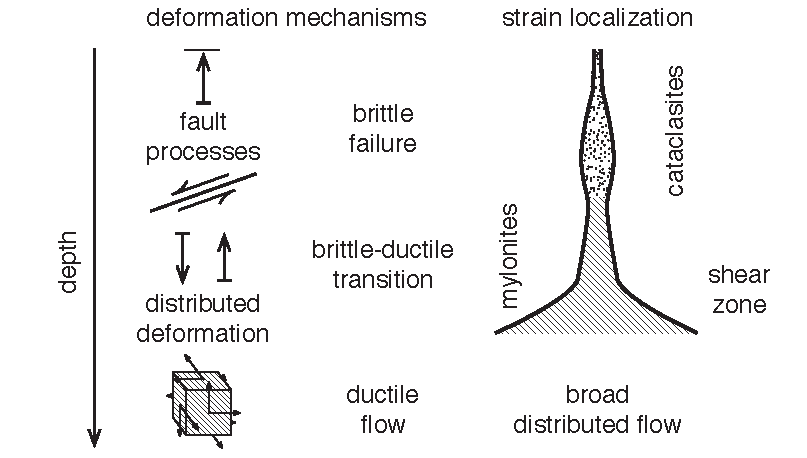
\includegraphics[width=1\textwidth]{strain-localization}
\end{center}
\vspace{-0.5cm}
\end{figure}
%
\\
Viscoelastic relaxation plays an important role during the seismic cycle, as these transients create a time-dependent stress transfer that can affect the loading rate of distant faults. These \textbf{long-range interactions} can modulate the recurrence times of earthquakes. As discussed in the previous chapter, aseismic fault processes are competing mechanisms of stress transfer, and in general it is important to consider all these mechanisms of deformation together, so that their individual effect can be singled out. For example, a low mantle viscosity can be mistakingly inferred from postseismic deformation modeling, when the deformation is in fact due to deep afterslip on the down-dip extension of the ruptured fault, or vice-versa. 


\section{Strength of the lithosphere}

In regions of high viscosity, the maximum stress is controlled by the \textbf{yield stress} of rocks for \textbf{brittle failure}. Rocks break when the shear stress reaches a yield stress, which is well described by the experiments of \cite{byerlee78a}. The yield stress increases linearly with effective confining pressure following the Coulomb friction law $\tau^\text{yield}=\mu_0\bar{\sigma}$, with the static friction coefficient $\mu_0=0.85$. In the case of low viscosity, rocks deform viscously before they break, so depending on the physical conditions (mostly temperature) there is a competition between deformation by distributed flow or localized failure along faults. The point where rocks could equally fail macroscopically or flow viscously is called the \textbf{brittle-ductile transition}. Understanding the depth dependence of viscosity is important to understand the thickness of the rigid plate and its deformation style.

\subsection{Diffusion and dislocation creep}

The \textbf{strength of the lithosphere} represents the maximum shear stress that the rocks can support at steady state before flowing or breaking. The strength of the lithosphere is controlled by its weakest and most pervasive elements. In the oceanic upper mantle, the strength envelope is controlled by the properties of olivine. In continents, the rheology of quartzite defines the strength of the crust, and the properties of olivine are used for the mantle. The flow laws are derived from laboratory experiments. They indicate that Earth's rocks deform under three main regimes: \textbf{diffusion creep}, \textbf{dislocation creep} and the \textbf{Peierls mechanism}. The Peierls mechanism is occurring at high stress levels, physically representing the yield stress of the material, and is not ubiquitous in the earth. However, the Peierls mechanism may be important for the deformation of shear zones, near the brittle-ductile transition. Its effect on the strength of the lithosphere is not considered important. The two other mechanisms take place simultaneously, 
\begin{equation}
\dot{\epsilon}^i\,=~\dot{\epsilon}^\text{diffusion}+\dot{\epsilon}^\text{dislocation}
\end{equation}
and they represent a combination of various \textbf{micro-mechanisms} of deformation (dislocation climb, grain-boundary sliding, grain-boundary diffusion, pressure-solution creep). The dominant regime is dictated by the ambient stress conditions: diffusion creep for low stress conditions and dislocation creep for high stress conditions.\\
\\
Diffusion creep gives rise to a linear stress/strain-rate relationship of the form
\begin{equation}
\dot{\epsilon}^\text{diffusion}=A\,\tau\,d^{-p}\,\big(C_\text{OH}\big)^r\,\exp\left(\alpha\phi\right)\,\exp\left(-\frac{Q+pV}{RT}\right)
\end{equation}
where $A$ is a reference strain rate, $\tau$ is the shear stress, $d$ is the grain size, $C_\text{OH}$ is the water concentration, $\phi$ is the melt fraction, $Q$ is the activation energy, $p$ is the ambient pressure, $V$ is the activation volume, and $T$ is the temperature in Kelvin. In addition, $R$ is the universal gas constant, and $p$ and $r$ are power exponents. This seems complicated, but really all it is saying is that
\begin{equation}
\dot{\epsilon}^\text{diffusion}=\frac{\tau}{\eta^\text{diffusion}}
\end{equation}
What the experimentalists have been able to accomplish is to predict the value of viscosity based on physical conditions
\begin{equation}
\eta^\text{diffusion}=\frac{1}{A}\,d^{p}\,\big(C_\text{OH}\big)^{-r}\,\exp\left(-\alpha\phi\right)\,\exp\left(\frac{Q+pV}{RT}\right)
\end{equation}
The typical values for these parameters are compiled by \cite{hirth&kohlstedt03} and \cite{burgmann&dresen08} and are summarized for the diffusion creep for olivine and quartz in Table \ref{tbl:linear-viscosity}.\\ 
%
\begin{table}[t]
\centering
\def\arraystretch{1.5}
\begin{tabular*}{1\columnwidth}{ccccccc}
 &        &        &       &                & $Q$ & $V$ \\
 & $\text{log}_{10}\,A$ & $p$ & $r$ & $\alpha$ & (kJ/mol) & ($10^{-6}$m$^3$/mol) \\
\hline
Olivine \\
Dry diffusion & $+9.2\pm0.2$  & $3$ & 0 & $30$ & $375\pm50$ & $2-10$ \\
Wet diffusion & $+6.0\pm0.2$  & $3$ & 1.0 & 30 & $335\pm75$ & $1-10$ \\
Quartz \\
Wet diffusion & $-0.4\pm2.1$  & $2\pm0.8$ & 1.0 & - & $220\pm55$ & - \\
\end{tabular*}
\vspace{0.1cm}
\caption{Physical parameters for diffusion creep for crust (quartz) and upper-mantle (olivine) conditions. A typical value for grain size is $d=10^4\,\mu$m. Dry conditions apply for $C_\text{OH}\le50\,$H/$10^{6}$Si. The shear stress is in MPa and the strain rates are in /s.}
\label{tbl:linear-viscosity}
\end{table}
\\
Diffusion creep is sensitive to \textbf{partial melting}. But for earthquake studies, the partial melt content is oftentimes $\phi=0$. (The effect of partial melting is more relevant for volcanic or other shallow processes.) Over long time scales, the grain size can evolve, leading to \textbf{strain weakening} for grain-size reduction and \textbf{strain hardening} for grain-size increase.\\
\\
Dislocation creep creates a nonlinear stress/strain-rate relationship where the strain rate is proportional to the shear stress raised to a power
\begin{equation}
\dot{\epsilon}^\text{dislocation}=A\,\tau^n\,\big(C_\text{OH}\big)^r\,\exp\left(\alpha\phi\right)\,\exp\left(-\frac{Q+pV}{RT}\right)
\end{equation}
where $n$ is the power exponent for stress. The nonlinear stress dependence emerges because the strain rate depends on both the internal dislocation density and the slip rate on individual dislocations; and both increase with stress. For dislocation creep, there is no dependence on grain size. We can still write the power-law rheology with an effective viscosity. In this case the effective viscosity depends on stress
\begin{equation}
\eta^\text{dislocation}=\frac{1}{A}\tau^{1-n}\,\big(C_\text{OH}\big)^{-r}\,\exp\left(-\alpha\phi\right)\,\exp\left(\frac{Q+pV}{RT}\right)
\end{equation}
The values for these physical parameters in the dislocation creep regime are given is Table~\ref{tbl:powerlaw-viscosity}. Values of activation volume are not well defined for quartz, but the effect of pressure is minimal in crustal conditions.\\
%
\begin{table}[t]
\centering
\captionwidth{0.78\linewidth}
\def\arraystretch{1.5}
\begin{tabular*}{0.98\columnwidth}{ccccccc}
 &        &        &       &                & $Q$ & $V$ \\
 & $\text{log}_{10}\,A$ & $n$ & $r$ & $\alpha$ & (kJ/mol) & ($10^{-6}$m$^3$/mol) \\
\hline
Olivine \\
Dry dislocation & $+5.0\pm0.2$ & $3.5$  & 0 & $30$ & $530\pm4$ & $18$ \\
Wet dislocation & $+3.2\pm0.2$ & $3.5$ & 1.0 & 30 & $520\pm40$ & $22\pm11$ \\
Quartz \\
Wet dislocation & $-4.9\pm0.4$ & $3.0$ & 1.0 & - & $242\pm24$ & - \\
Feldspar \\
Dry dislocation & $+12.7\pm0.2$ & $3.0$ & 0 & - & $641$ & $24$
\end{tabular*}
\vspace{0.1cm}
\caption{Physical parameters for dislocation creep for crust (quartz \& feldspar) and upper-mantle (olivine) conditions 	from \cite{hirth&kohlstedt03} and \cite{burgmann&dresen08}.}
\label{tbl:powerlaw-viscosity}
\end{table}
%
\\
For the Peierls mechanism the activation enthalpy depends on stress and a rheology of the form
\begin{equation}
\dot{\epsilon}^\text{Peierls}=A\left[\sinh\left(\frac{\tau}{G}\right)\right]^n\,\exp\left(-\frac{Q}{RT}\right)
\end{equation}
applies. Note the resemblance of this expression to the constitutive expression for fault slip under the rate-strengthening approximation.


\subsection{Strength-envelope diagram}

\begin{figure}[p]
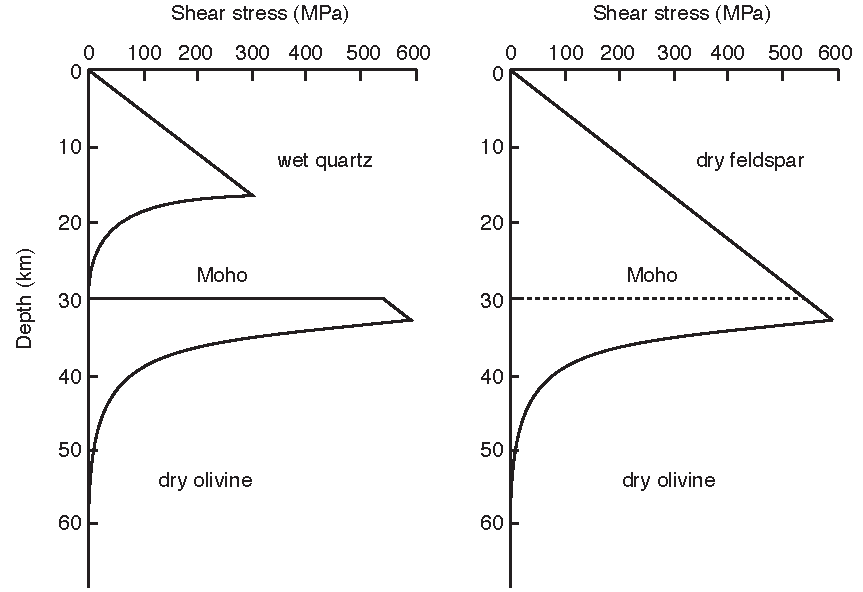
\includegraphics[width=1\columnwidth]{jelly-sandwich_creme-brulee}
\caption{Strength envelopes for the continental lithosphere. Left) Jelly sandwich model with a weak lower crust due to a wet quartz rheology. The upper-most mantle is strong and forms a rigid lid. Right) Cr\`{e}me-br\^{u}l\'{e}e model with a strong crust due to a dry feldspar rheology. The models assume dislocation creep with a strain rate of $\dot{\epsilon}^i=10^{-14}\,$s$^{-1}$, after \cite{burgmann&dresen08}.}
\label{fig:strenth-envelope-continent}
\end{figure}
%
The mechanical properties of crustal and mantle materials allow us to predict the stress in the lithosphere assuming a strain rate ($\tau=\eta_\text{effective}\,\dot{\epsilon}^i$). The model is based on a thermal profile of the lithosphere based on \textbf{thermal diffusion} from the basal temperature $T_m$ to the surface $T_0=0$, as follows
\begin{equation}
T(x_3,t)=T_m\text{erf}\left(\frac{x_3}{2\sqrt{K t}}\right)
\end{equation}
where $\text{erf}(x)$ is the error function, $x_3$ is depth, $T_m$ is the temperature at the base of the upper mantle, 
\begin{equation}
K=\frac{k}{\rho_mC_p}
\end{equation}
is the thermal diffusivity in m$^2$/s, $k=3.138\,$W/m/K is the thermal conductivity, $C_p=1.17\times10^{3}\,$J/kg/K is the specific heat and $\rho_m=3.33\times10^{3}\,$kg/m$^3$ is the mantle mass density. The mantle basal temperature is poorly constrained and estimates vary between $1300^\circ$C and $1450^\circ$C. As thermal weakening plays an important role in the rheology of olivine, uncertainties in basal temperature imply large uncertainties in effective viscosity or lithosphere strength in the mantle.\\
%
\\
Based on reasonable assumptions about the thermal profile, there are two end-member models about the strength of the continental lithosphere. In the \textbf{``jelly-sandwich''} model, the lower crust is weak, for example controlled by the quartzite rheology under wet conditions. The change of lithology from crustal to mantle rocks at the Moho creates a strong upper mantle. Therefore the lower crust is ``sandwiched'' between two strong layers and the lower crust is the ``jelly''. In the \textbf{``cr\`{e}me-br\^{u}l\'{e}e''} model, the lower crust is strong, as if controlled by the dry feldspar rheology and the distributed flow only occurs in the upper mantle. The strong layer above a soft paste reminds us of the delicious French dessert! The stress is always lower than the brittle resistance of rocks, which creates a wedge of increasing stress. Because of the particular shape of the strength envelope, it is affectionally called a \textbf{``Christmas-tree''} diagram.

\clearpage
\subsection{The oceanic lithosphere}

The oceanic lithosphere has a simpler thermal structure and composition than the continental lithosphere. The oceanic crust is less than 10\,km thick and therefore most of the oceanic lithosphere strength is controlled by the mechanical properties of olivine. The variations of strength span a range of several orders of magnitude so it is convenient to draw the Christmas-tree diagram in logarithm scale (Figure~\ref{fig:asthenosphere}). For much of the depths of the upper mantle, temperature increases quasi-linearly. This gives rise to an exponential decrease of the effective viscosity with depth. Low effective viscosities are attained at great depths, around 80\,km. But as temperature gradients decrease around 100\,km depth, thermal weakening starts to be compensated by pressure hardening. The competition between thermal weakening and pressure hardening controls the depth and the thickness of the asthenosphere. \\
\begin{figure}[h]
\centering
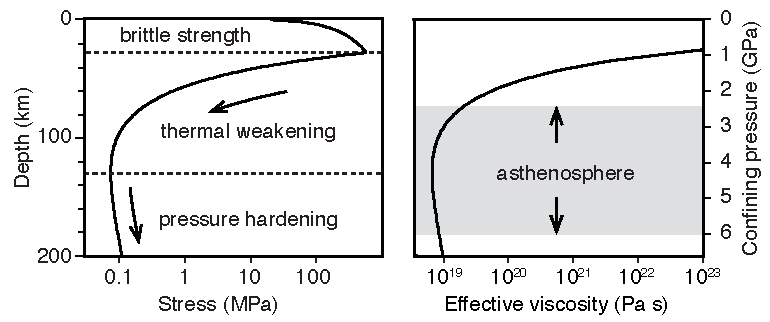
\includegraphics[width=1\columnwidth]{oceanic-lithosphere-log}
\caption{Strength and effective viscosity of the oceanic lithosphere (t=60\,Myr, V=17\,cm$^3$/mol). The oceanic upper mantle is strong and can accommodate faulting to great depths. The depth and thickness of the asthenosphere is controlled by the relative effects of thermal weakening and pressure hardening.}
\label{fig:asthenosphere}
\end{figure}
%
\\
Geodetic studies of the mechanical properties of the oceanic asthenosphere in the context of postseismic deformation can place constraints on the depth and the thickness of low-viscosity regions. However, the strength envelope only represents the shear stress in the lithosphere at \textbf{steady state} and it ignores the effect of stress modulations from the earthquake cycle. One way to describe the properties of the lithosphere that is relevant during both steady state and postseismic transients is the fluidity for dislocation creep
\begin{equation}
\dot{\gamma}_0=A\,G^{n}\,\big(C_\text{OH}\big)^r\,\exp\left(\alpha\phi\right)\,\exp\left(-\frac{Q+pV}{RT}\right)
\end{equation}
i.e., we have $\epsilon^i=\dot{\gamma}_0\left(\tau/G\right)^n$. Fluidity is a reference strain rate and it controls the inelastic strain rate both during steady state and transients. The effect of basal temperature, plate age, water, and activation volume on fluidity are shown in Figure~\ref{fig:fluidity}. The physical parameters that have simultaneously the most effect on fluidity and the most uncertainties are the upper-mantle basal temperature, the water content and the activation volume. Geophysical studies should target these parameters to complement laboratory studies. Activation volume controls the depth and thickness of the asthenosphere. A change of a few degrees in basal temperature or in water content can change the strain rate significantly.\\
%
\begin{sidewaysfigure}[p]
\captionwidth{0.9\linewidth}
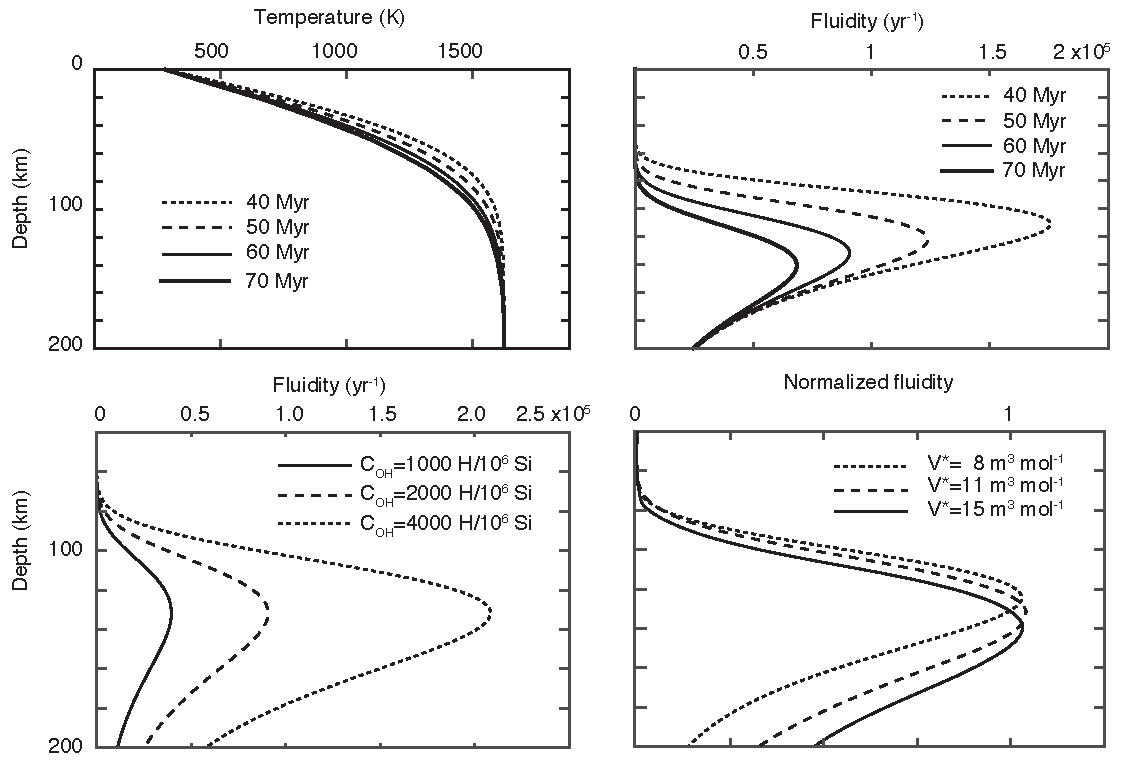
\includegraphics[width=\textwidth]{fluidity-ocean.pdf}
\caption{Effect of temperature, pressure and fluid content on olivine fluidity $\dot{\gamma}=\epsilon^i/\tau^n$. Top left) The thermal profiles for oceanic plates of 40, 50, 60 and 70\,Myr assuming a basal temperature of $T_m=1350^\circ$C. Top right) Effect of plate age on fluidity. Bottom left) Effect of water content. Right) Activation volume affects the depth and thickness of the asthenosphere.}
\label{fig:fluidity}
\end{sidewaysfigure}
%
\\
More thoughts and discussions:
1) Earthquake cycle considerations. Trade-offs with afterslip.
2) Newtonian fluid, power-law rheology.
3) Difference between linear and power-law relaxation in geodetic data: different time evolution, different vertical displacements. 
4) Transient effect?

%
\clearpage
\section{The spring-dashpot model}

To better understand the behavior of a viscoelastic material under a stress perturbation, we can approximate the mechanical system by a spring and dashpot in series. The \textbf{spring-dashpot} model can approximate a shear zone or the continental lower crust subject to the sudden shear stress perturbation caused by an earthquake in the brittle layer.
%
\begin{figure}[h]
\begin{center}
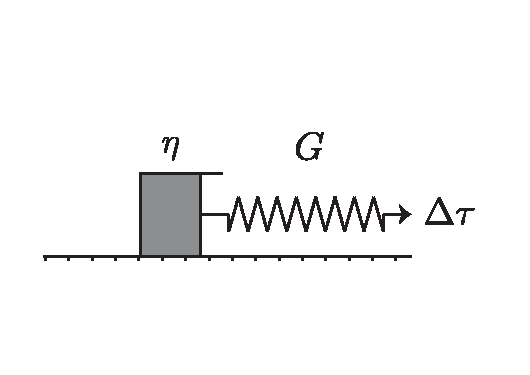
\includegraphics[width=0.5\textwidth]{spring-dashpot-setup}
\end{center}
\vspace{-0.5cm}
\end{figure}
%
The dashpot is a viscous material and the spring is elastic. The joint response of the system is viscoelastic. When the spring and the dashpot are put in series, the cumulative strain of the system is the sum of the elastic and viscous contributions. We will consider the case of the linear and power-law rheologies. \\
\\
In the case of diffusion creep, we simplify the stress/strain-rate relationship with $\dot{\epsilon}^i=\tau/\eta$. The evolution of shear stress is governed by the differential equation
\begin{equation}\label{eqn:power-law-creep}
\dot{\tau}+\frac{G}{\eta}\,\tau=0
\end{equation}
The solution is given by
\begin{equation}
\tau(t)=\tau_0\,e^{-t/t_m}
\end{equation}
where $\tau_m$ is the initial (coseismic) loading, and the time scale
\begin{equation}\label{eqn:linear_time_scale}
\boxed{\begin{aligned}
t_m=\frac{\eta}{G}
\end{aligned}}
\end{equation}
is called the \textbf{Maxwell time}, or \textbf{relaxation time}, of the viscoelastic transient. In a linear rheology, the Maxwell time is independent of the initial stress condition. \\
\\
As stress is relaxed, cumulative inelastic strain in the volume increases 
\begin{equation}\label{eqn:linear-strain}
\gamma(t)=\frac{\tau_0}{G}\left(1-e^{-t/t_m}\right)~.
\end{equation}
The displacement in the elastic medium should exhibit a similar time dependence, but the amplitude of displacement will decay away from the source. Geodetic studies are most sensitive to short relaxation times, which are caused by the relaxation of the lowest-viscosity material. For this reason, geodesy is best used to constrain the viscous properties of deep sources, where the effective viscosity is associated with relaxation times lower than a decade or so.\\
\\
For dislocation creep, we simplify the stress/strain-rate relationship by considering the flow law
\begin{equation}
\dot{\epsilon}^i=A\left(\frac{\tau}{G}\right)^n
\end{equation}
with $n>1$. In this case, the governing equation for the stress evolution is
\begin{equation}
\frac{\dot{\tau}}{G}+A\,\left(\frac{\tau}{G}\right)^{n}=0
\end{equation}
which solves for
\begin{equation}\label{eqn:power-law-decay}
\tau(t)=\tau_0\,\left[1+A\,(n-1)\,\left(\frac{\tau_0}{G}\right)^{n-1}t\right]^{\frac{-1}{n-1}}
\end{equation}
where the timescale of deformation $t_0$ now scales with the initial stress $\tau_0$
\begin{equation}\label{eqn:power-law_time_scale}
t_0=\frac{1}{A\,(n-1)}\,\left(\frac{G}{\tau_0}\right)^{n-1}
\end{equation}
so that large stress perturbations give rise to shorter transients. Integrating eq.~(\ref{eqn:power-law-creep}) and~(\ref{eqn:power-law-decay}), we obtain the evolution of inelastic strain\\
\begin{equation}\label{eqn:power-law-strain}
\gamma(t)=\frac{\tau_0}{G}\,\left(1-\left[1+\frac{t}{t_0}\right]^{\frac{-1}{n-1}}\right)
\end{equation}
%
Geodetic studies need to discriminate between the expected responses of linear and non-linear rheologies. The impulse response to an instantaneous stress change for the diffusion and disocation creep is illustrated in Figure~\ref{fig:creep-test}. Compared to the linear case most of the deformation for dislocation creep happens at an early time. But complete relaxation, however, takes a much longer time. \\
%
\begin{figure}[p]
\begin{center}
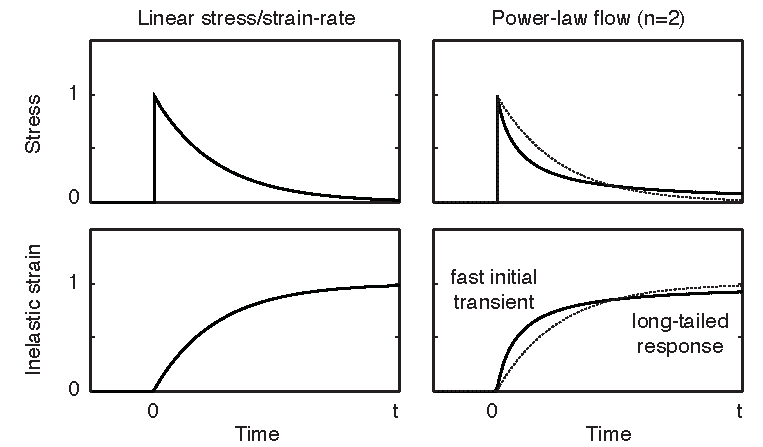
\includegraphics[width=1\textwidth]{impulse-response-viscoelastic}
\end{center}
\caption{Relaxation of a stress perturbation by a spring-dashpot system. With a non-linear rheology ($n=2$), the initial strain rate is higher than in the case of a linear rheology. But the later response is slower. Here, the stress is non-dimensionalized by $\Delta\tau_0$, and the inelastic strain, by $\tau_0/G$.}
\label{fig:creep-test}
\end{figure}
%\vspace{-0.5cm}
%
\\
The time evolution of the cumulative inelastic strain should resemble the one of the surface deformation at a given point. But the spring-dashpot model is an \"{u}ber-simplification only meant to inform intuition. In reality, the strain can be directed in six independent directions and the displacement at the surface of the Earth would be due to elastic deformation caused by a distant source. Geodesy measures the total deformation caused by both the viscous strain and the elastic coupling. 

\clearpage
\section{Viscoelastic deformation in a continuum}

The previous section described the temporal evolution of inelastic strain in a simple system. The \textbf{continuum description} of viscoelasticity is concerned with a representation of inelastic strain in three dimensions. So stress and strain are now second-order tensors representing forces and deformation in nine different directions. In a system of right-handed coordinates $(\textbf{e}_1, \textbf{e}_2, \textbf{e}_3)$, the Cauchy stress tensor $\sigma_{ij}$ represents the force couples applied on a surface $\textbf{e}_i$ and pointing in the direction $\textbf{e}_j$~\citep{malvern69a}.
%
\begin{figure}[h]
\centering
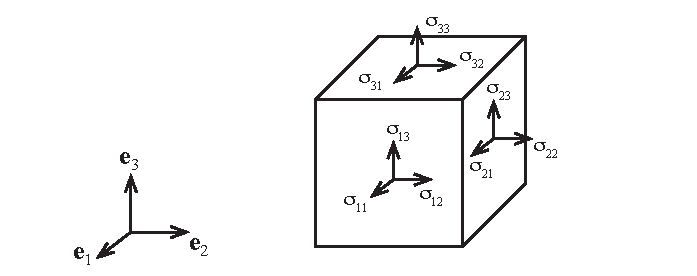
\includegraphics[width=0.9\columnwidth]{stress-tensor}
\end{figure}
Because stress is symmetric - this comes from conservation of angular momentum - the stress can be oriented in six independent directions. In this case, how can we relate stress and strain rate? \\
\\
In a viscoelastic material the total strain-rate tensor $\dot{\epsilon}_{ij}$ is the sum of the elastic and the inelastic contributions
%
\begin{equation}\label{eqn:total-strain_gen}
\dot{\epsilon}_{ij}=\dot{\epsilon}_{ij}^e+\dot{\epsilon}_{ij}^i
\end{equation}
%
where the dots represent time differentiation. Elastic materials obey Hooke's law, expressed here in tensor form 
\begin{equation}
\sigma_{ij}=C_{ijkl}\epsilon_{kl}^e
\end{equation}
where $C_{ijkl}$ is the fourth-order elastic moduli tensor and $\epsilon_{ij}^e$ is the elastic strain tensor. Or, reciprocally, we can write
\begin{equation}
\epsilon_{ij}^e=D_{ijkl}\sigma_{kl}
\end{equation}
where $D_{ijkl}$ is the fourth-order elastic compliance tensor. The inelastic strain rate follows the \textbf{constitutive relationship}
\begin{equation}\label{eqn:plastic-constitutive_gen}
\dot{\epsilon}^i_{ij}=\dot{\gamma}\,R_{ij}
\end{equation}
where $\gamma$ is the amplitude of inelastic strain and $R_{ij}$ is a unitary ($R_{kl}R_{kl}=1$) and symmetric ($R_{ij}=R_{ji}$) tensor representing the direction of the inelastic strain rate. In general the inelastic strain rate is subject to a flow law of the form
\begin{equation}\label{eqn:general_evolution_law_gen}
\dot{\gamma}=f(\sigma_{ij},\gamma)
\end{equation}
where $\sigma_{ij}$ is the Cauchy stress and $\gamma$ is the cumulative amplitude of inelastic strain. The presence of $\gamma$ in the evolution law (\ref{eqn:general_evolution_law_gen}) is justified to represent the effects of \textbf{work strengthening} or \textbf{work weakening}. \\
\\
The particular form of operator $f$, which is referred to as a rheology, depends upon the source mechanism. When no work hardening takes place the rheology $\dot{\gamma}=f(\sigma_{ij})$ is an algebraic equation. If the instantaneous inelastic strain rate depends on the history of deformation, then the rheology $\dot{\gamma}=f(\sigma_{ij},\gamma)$ is a differential equation coupled to the equation for stress evolution. \\
\\
For diffusion and dislocation creep, the stress/strain-rate constitutive relation can be written in the form
\begin{equation}
\dot{\gamma}=\dot{\gamma}_0\left(\frac{\tau}{G}\right)^{n}
\end{equation}
where $\dot{\gamma}_0$ is the fluidity, $n$ is the stress power exponent and $G$ is the shear modulus. Here, $\tau$ is the amplitude (or norm) of the deviatoric stress tensor
\begin{equation}
\sigma'_{ij}=\sigma_{ij}-\delta_{ij}\frac{\sigma_{kk}}{3}
\end{equation} 
so the shear stress is simply
\begin{equation}
\tau=\big|\big|\boldsymbol{\sigma}'\big|\big|=\left(\frac{1}{2}\sigma'_{kl}\sigma'_{kl}\right)^{1/2}
\end{equation} 
In simple models of viscoelastic deformation, we assume that the stress and strain rate are co-aligned, and that there are no volumetry strain rate. So the strain-rate tensor is purely deviatoric. The direction of the strain rate tensor is therefore the same as the deviatoric stress tensor
\begin{equation}
R_{ij}=\frac{\sigma'_{ij}}{\tau}
\end{equation}
In the end the constitutive relationship can be written
\begin{equation}
\dot{\epsilon}_{ij}^i=\dot{\gamma}_0\left(\frac{\tau}{G}\right)^{n-1}\frac{1}{G}\,\sigma'_{ij}
\end{equation}
but in general it is simpler to think about the amplitude and the direction of the constitutive relationship separately. Other, more complicated, constitutive relationships can be derived to include the effect of \textbf{plastic anisotropy} or state variables can be added to represent, for example, the effect of \textbf{grain size evolution}.


\subsection{Effect of prestress on nonlinear rheologies}

Since nonlinear rheologies like the power-law flow are sensitive to the absolute value of stress, it is necessary to include both the effects of the stress change brought by a nearby earthquake (or another stress perturbation) and of the \textbf{background stress}, or \textbf{prestress}. However, to model postseismic deformation time series, it is convenient to simulate only the perturbation to the background strain rate, as the background strain rate itself does not affect the stress. \\
\\
The absolute value of shear stress is
\begin{equation}
\tau=\big|\big|\bar{\boldsymbol{\sigma}}+\boldsymbol{\sigma}'\big|\big|
\end{equation}
and the background shear stress
\begin{equation}
\tau_0=\big|\big|\bar{\boldsymbol{\sigma}}\big|\big|
\end{equation}
where $\bar{\boldsymbol{\sigma}}$ is the background deviatoric stress tensor and $\boldsymbol{\sigma}'$ is the deviatoric stress change tensor. One can define the following flow law
\begin{equation}
\dot{\epsilon}_{ij}^i=\dot{\gamma}_0\left(\frac{\tau}{G}\right)^{n-1}\frac{1}{G}\,\left(\bar{\sigma}_{ij}+\sigma'_{ij}\right)-\dot{\gamma}_0\left(\frac{\tau_0}{G}\right)^{n-1}\frac{1}{G}\,\bar{\sigma}_{ij}
\end{equation}
The first term is the total inelastic strain rate and the second term is the background strain rate. When the stress perturbation has been relaxed, i.e., when $\big|\big|\boldsymbol{\sigma}'\big|\big|=0$, the postseismic strain rate vanishes.

\section{Green's function method}

Assuming infinitesimal strain, combining eqs.~(\ref{eqn:total-strain_gen}) to~(\ref{eqn:plastic-constitutive_gen}) and integrating, we obtain the general \textbf{hereditary equation} for stress evolution
%
\begin{equation}\label{eqn:stress-time_gen}
\sigma_{ij}(t)=C_{ijkl}\epsilon_{kl}(t)-\int_0^t\,\dot{\gamma}(\tau)\,C_{ijkl}R_{kl}(\tau)\,d\tau
\end{equation}
%
where $\tau$ is a dummy variable of the time integration. In a viscoelastic material the stress is reduced by its history of inelastic deformation. Eq.~(\ref{eqn:stress-time_gen}) reduces to a linear combination of strain components, i.e. Hooke's law for a simple elastic material, if no inelastic deformation occurs. The total strain $\epsilon_{ij}$ can simply be evaluated from the current state of deformation 
%
\begin{equation}\label{eqn:gradient}
\begin{aligned}
\epsilon_{ij}(t)&=\frac{1}{2}\left(u_{i,j}+u_{j,i}\right)
\end{aligned}
\end{equation}
%
where the current displacement field records a history of deformation
%
\begin{equation}\label{eqn:displacement-velocity}
u_i(t)=u_i(0)+\int_0^tv_i(\tau)\,d\tau
\end{equation}
%
Similarly the rate of change of stress, $\dot{\sigma}_{ij}=C_{ijkl}\dot{\epsilon}_{kl}^e$ can be written using eq.~(\ref{eqn:total-strain_gen})
\begin{equation}\label{eqn:stress_rate_gen}
\dot{\sigma}_{ij}=C_{ijkl}\big(\dot{\epsilon}_{kl}-\dot{\epsilon}_{kl}^i\big)
\end{equation}
where we recognize the instantaneous power -strictly speaking, the power density- by internal processes of inelastic deformation
\begin{equation}\label{eqn:torque_density_rate_gen}
\dot{m}_{ij}=C_{ijkl}\,\dot{\epsilon}_{kl}^i
\end{equation}
The instantaneous power~(\ref{eqn:torque_density_rate_gen}) is homogeneous to a moment-density rate and is a forcing term in tensor space. \\
\\
A time series of deformation can be evaluated given a specific rheology in the form of eq.~(\ref{eqn:general_evolution_law_gen}). At all times, a displacement field must satisfy the condition of vanishing of surface traction
\begin{equation}\label{eqn:vanishing_traction_gen}
\int_{\partial\Omega}\sigma_{ij}(t)\,\hat{n}_j\,dA=0
\end{equation}
The criterion~(\ref{eqn:vanishing_traction_gen}) is satisfied by enforcing simultaneously a free surface boundary condition $\dot{\sigma}_{ij}\hat{n}_{j}=0$ and the conservation of the rate of momentum $\dot{\sigma}_{ij,j}=0$. Using~(\ref{eqn:stress_rate_gen}) and~(\ref{eqn:torque_density_rate_gen}) the free-surface boundary condition becomes
\begin{equation}\label{eqn:surface_boundary_condition_gen}
\dot{t}_i=C_{ijkl}\,\dot{\epsilon}_{kl}\,\hat{n}_j=\dot{m}_{ij}\,\hat{n}_j
\end{equation}
where $\hat{n}_i$ is the normal vector at the surface $\partial\Omega$. Eq.~(\ref{eqn:surface_boundary_condition_gen}) indicates that a postseismic source mechanism contributes to some equivalent rate of surface traction $\dot{t}_i$ if the corresponding eigenstrain-rate $\dot{\epsilon}_{ij}^i$ is non-zero at the surface $\partial\Omega$. Without loss of generality, the conservation of rate of momentum can be written
\begin{equation}\label{eqn:cons_mom_gen}
\left(C_{ijkl}\,\dot{\epsilon}_{kl}\right)_{,j}+\dot{f}_i=0
\end{equation}
which corresponds to the inhomogeneous Navier's equation in the case of a homogeneous isotropic elastic solid and where we have defined the body-force rate
\begin{equation}\label{eqn:general_body_force_gen}
\dot{f}_i=-\dot{m}_{ij,j}
\end{equation}
The mechanisms driving a post earthquake transient can be equivalently represented by the eigenstrain-rate of eq.~(\ref{eqn:plastic-constitutive_gen}), the power density of eq.~(\ref{eqn:torque_density_rate_gen}) and the distribution of equivalent body force and surface traction rate of eqs.~(\ref{eqn:general_body_force_gen}) and (\ref{eqn:surface_boundary_condition_gen}), respectively. \\
\\
A time series of transient deformation following a stress perturbation can be obtained as follows. From a given level of stress at time $t$, we evaluate the eigenstrain rate due to a particular mechanism with eq.~(\ref{eqn:plastic-constitutive_gen}). We evaluate the corresponding power density~(\ref{eqn:torque_density_rate_gen}) and compute the associated distribution of surface traction and internal forces with eq.~(\ref{eqn:surface_boundary_condition_gen}) and~(\ref{eqn:general_body_force_gen}) respectively. We then solve eq.~(\ref{eqn:cons_mom_gen}) for a velocity field. We obtain the new displacement, stress, and cumulative strain fields for time $t+dt$ by integrating the corresponding quantities in the time domain using an explicit method with a predictor/corrector scheme. In particular, the stress-tensor field at $t+dt$ is obtained form eq.~(\ref{eqn:stress-time_gen}). We repeat these steps until the simulation of the viscoelastic relaxation over a specified time interval is complete. \\
\\
One important aspect of the representation of postseismic mechanisms in terms of equivalent body forces is that regardless of how nonlinear the form of a viscous rheology can take, the 3-D instantaneous velocity field remains the solution of a linear partial differential equation. The velocity field satisfies the inhomogeneous Navier's equation~(\ref{eqn:cons_mom_gen}) with the inhomogeneous boundary condition (\ref{eqn:surface_boundary_condition_gen}) and the methods to solve elasto-static problems become applicable to evaluate models of nonlinear time-dependent deformation.\\
\\
The instantaneous velocity field $v_i$ can in general be obtained with application of the elastic Green's function
\begin{equation}\label{eqn:velocity_greens}
\begin{aligned}
v_i(x_i)&=\int_{\Omega}G_{ij}(x_i,y_i)\,\dot{f}_j(y_i)\,dV\\
&\qquad\qquad+~\int_{\partial\Omega}G_{ij}(x_i,y_i)\,\dot{t}_j(y_i)\,dA\
\end{aligned}
\end{equation}
Interestingly, the details of the geometry and the elastic structure of the viscoelastic body are all captured by the specific form of the elastic Green's function $G_{ij}$. The Green's function for a semi-infinite solid is described by~\cite{love27} and~\cite{nemat-nasser&hori99}. The Green's function with gravitational effects is detailed by~\cite{pollitz97a} for a layered spherical body and by~\cite{wang+03a} for a layered half space. In general the distribution of internal body force can occupy a large volume and the method that consists in performing the convolution between the Green's function and the forcing terms can be impractical. This difficulty can be alleviated by using a Fourier-domain elastic Green's function~\citep{barbot+09a,barbot+09b} or by discretizing eq.~(\ref{eqn:velocity_greens}) in finite volumes, as described below, and using the integral method to solve the time-dependent problem.


\clearpage
\section{Green's functions for distributed inelastic strain of finite volumes}

\subsection{Antiplane strain in a half space}

We consider the distributed strain occurring in an elementary rectangular volume. Let's start with the reference system $(0,\textbf{e}_1,\textbf{e}_2,\textbf{e}_3)$. In two-dimensional, antiplane, strain, $\partial/\partial x_1=0$ and $u_2=u_3=0$. We consider a rectangular area of length $L$ and width $W$ at depth $D$. 
%
\begin{figure}[h]
\centering
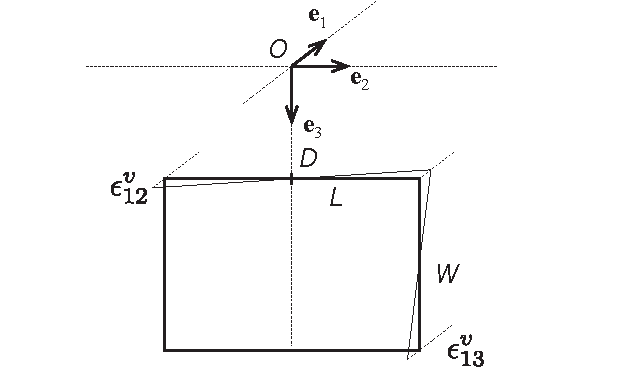
\includegraphics[width=0.6\columnwidth]{geometry-antiplane.pdf}
\end{figure}
% 


The area is subjected to the eigenstrain
\begin{equation}
\boldsymbol{\epsilon}^v=\left(\begin{matrix}
0 & \epsilon_{12}^v & \epsilon_{13}^v\\
\epsilon_{21}^v & 0 & 0\\
\epsilon_{31}^v & 0 & 0\\
\end{matrix}\right)
\end{equation}
(with $\epsilon_{21}=\epsilon_{12}$ and $\epsilon_{13}=\epsilon_{31}$.) This gives rise to the moment density tensor
\begin{equation}
\textbf{m}=\textbf{C}: \boldsymbol{\epsilon}^v=\left(\begin{matrix}
0 & m_{12} & m_{13}\\
m_{21} & 0 & 0\\
m_{31} & 0 & 0\\
\end{matrix}\right)=\left(\begin{matrix}
0 & 2G\epsilon_{12}^v & 2G\epsilon_{13}^v\\
2G\epsilon_{21}^v & 0 & 0\\
2G\epsilon_{31}^v & 0 & 0\\
\end{matrix}\right)
\end{equation} 
The deformation in the plane due to elastic coupling can be attributed to the equivalent body forces
\begin{equation}
\begin{aligned}
\textbf{f}&=-\nabla\cdot\textbf{m}\\
&=-2G\left[\epsilon_{12,2}^v+\epsilon_{13,3}^v\right]\,\textbf{e}_1
\end{aligned}
\end{equation}
The spatial extent of the eigenstrain can be defined with the generalized function $\Pi(x)$, the boxcar function, with $\Pi'(x)=\delta(x+1/2)-\delta(x-1/2)$. We have the eigenstrain distribution\\
\begin{equation}
\epsilon_{12}^v(\textbf{x})= \epsilon_{12}^v\,\Pi\left(\frac{x_2}{L}\right)\Pi\left(\frac{x_3-D}{W}-\frac{1}{2}\right)
\end{equation}
So we have the equivalent body forces
\begin{equation}
\begin{aligned}
f_1=2G\bigg[&\epsilon_{12}^v\frac{1}{L}\left(\delta\left(\frac{x_2}{L}-\frac{1}{2}\right)-\delta\left(\frac{x_2}{L}+\frac{1}{2}\right)\right)\Pi\left(\frac{x_3}{W}\right)\\
+&\epsilon_{13}^v\,\Pi\left(\frac{x_2}{L}\right)\frac{1}{W}\left(\delta\left(\frac{x_3-D-W}{W}\right)-\delta\left(\frac{x_3-D}{W}\right)\right)\bigg]
\end{aligned}
\end{equation}
with $f_2=f_3=0$. \\
%
\\
We consider the effect of the free surface. For antiplane strain, this can be achieved using the method of images, whereby any source in $x_3>0$ is paired by an image at $-x_3$ with the same force orientation in the $\textbf{e}_1$ direction. At the surface the normal stress, $\sigma_{13}=G u_{1,3}=0$ by construction. We implement this by considering the antiplane Green's function for a half space\\
\begin{equation}
u_1(x_2,x_3)=\frac{1}{2\pi}\bigg[\ln\left({x_2}^2+(x_3-y_3)^2\right) + \ln\left({x_2}^2+(x_3+y_3)^2\right)\bigg]
\end{equation}
for a point source at depth $y_3$. Then the displacements are
\begin{equation}
\begin{aligned}
u_1(x_2,x_3)=&\frac{-1}{2\pi G}\iint_{-\infty}^\infty f_1(y_2,y_3)\ln\left((x_2-y_2)^2+(x_3-y_3)^2\right)\diff y_2\diff y_3\\
&\frac{-1}{2\pi G}\iint_{-\infty}^\infty{f_1(y_2,y_3)\ln\left((x_2-y_2)^2+(x_3+y_3)^2\right)}\diff y_2\diff y_3
\end{aligned}
\end{equation}
The rectangular area where the eigenstrain is applied is between the depth $D$ and $D+W$ and centered on the origin. Expanding the equivalent body force, we define the following integrals
\begin{equation}
\begin{aligned}
J_{12}(x_2,x_3)=&
 \frac{\epsilon_{12}^v}{\pi}\int_{D}^{D+W} \ln\left((x_2+L/2)^2+(x_3-y_3)^2\right)\diff y_3\\
-&\frac{\epsilon_{12}^v}{\pi}\int_{D}^{D+W} \ln\left((x_2-L/2)^2+(x_3-y_3)^2\right)\diff y_3\\
\end{aligned}
\end{equation}
\begin{equation}
\begin{aligned}
K_{12}(x_2,x_3)=&\frac{\epsilon_{12}^v}{\pi}\int_{D}^{D+W} \ln\left((x_2+L/2)^2+(x_3+y_3)^2\right)\diff y_3\\
-&\frac{\epsilon_{12}^v}{\pi}\int_{D}^{D+W} \ln\left((x_2-L/2)^2+(x_3+y_3)^2\right)\diff y_3\\
\end{aligned}
\end{equation}
\begin{equation}
\begin{aligned}
J_{13}(x_2,x_3)=&\frac{\epsilon_{13}^v}{\pi}\int_{-L/2}^{L/2} \ln\left((x_2-y_2)^2+(x_3-D)^2\right)\diff y_2\\
-&\frac{\epsilon_{13}^v}{\pi}\int_{-L/2}^{L/2} \ln\left((x_2-y_2)^2+(x_3-D-W)^2\right)\diff y_2\\
\end{aligned}
\end{equation}
\begin{equation}
\begin{aligned}
K_{13}(x_2,x_3)=&\frac{\epsilon_{13}^v}{\pi}\int_{-L/2}^{L/2} \ln\left((x_2-y_2)^2+(x_3+D)^2\right)\diff y_2\\
-&\frac{\epsilon_{13}^v}{\pi}\int_{-L/2}^{L/2} \ln\left((x_2-y_2)^2+(x_3+D+W)^2\right)\diff y_2\\
\end{aligned}
\end{equation}
such that the displacement field is simply
\begin{equation}
 u_1(x_2,x_3)=J_{12}+K_{12}+J_{13}+K_{13}
\end{equation}
The integrals are given in explicit form below. They involve distance to the four corners of the rectangular area and their image. The terms $J_{12}$ and $J_{13}$ also appear for the full space solution.
 \begin{equation}
 \begin{aligned}
J_{12}= \frac{\epsilon_{12}^v}{\pi} \bigg[~&
\left( x_3-D-W \right) \ln\left((x_2-L/2)^2+(x_3-D-W)^2\right)\\
-& \left( x_3-D-W\right) \ln\left((x_2+L/2)^2+(x_3-D-W)^2\right)\\
-& \left(x_3-D\right) \ln\left((x_2-L/2)^2+(x_3-D)^2\right)\\
+&\left(x_3-D\right) \ln\left((x_2+L/2)^2+(x_3-D)^2\right)\\
+& 2\left( x_2-L/2 \right)\left(\arctan\frac {x_3-D-W}{x_2-L/2}-\arctan\frac {x_3-D}{x_2-L/2}\right)\\
+& 2\left( x_2+L/2 \right)\left(\arctan\frac {x_3-D}{x_2+L/2}-\arctan\frac {x_3-D-W}{x_2+L/2}\right)~ \bigg]
 \end{aligned}
 \end{equation}
 %
 \begin{equation}
 \begin{aligned}
J_{13}=\frac{\epsilon_{13}^v}{\pi}\, \bigg[~&
   \left(x_2-L/2\right) \ln \left((x_2-L/2)^2+(x_3-D-W)^2\right)\\
-& \left(x_2+L/2\right) \ln \left((x_2+L/2)^2+(x_3-D-W)^2\right)\\
-& \left(x_2-L/2\right) \ln \left((x_2-L/2)^2+(x_3-D)^2\right)\\
+& \left(x_2+L/2\right) \ln \left((x_2+L/2)^2+(x_3-D)^2\right)\\
+& 2\left(x_3-W-D\right)\left(\arctan\frac {x_2-L/2}{x_3-D-W}-\arctan\frac {x_2+L/2}{x_3-D-W}\right)\\
+& 2\left(x_3-D\right) \left(\arctan\frac {x_2+L/2}{x_3-D}-\arctan\frac {x_2-L/2}{x_3-D}\right)\bigg] 
 \end{aligned}
 \end{equation}
The terms $K_{12}$ and $K_{13}$ come from the method of images.
 \begin{equation}
 \begin{aligned}
K_{12}=\frac{\epsilon_{12}^v}{\pi}\bigg[~&
 \left( x_3+D+W \right) \ln \left((x_2+L/2)^2+(x_3+D+W)^2\right)\\
-&\left( x_3+D+W \right) \ln \left((x_2-L/2)^2+(x_3+D+W)^2\right)\\
-& \left( x_3+D \right) \ln \left((x_2+L/2)^2+(x_3+D)^2\right)\\
+& \left( x_3+D \right) \ln \left((x_2-L/2)^2+(x_3+D)^2\right)\\
+& 2\left( x_2+L/2 \right) \left(\arctan \frac {x_3+D+W}{x_2+L/2}-\arctan \frac {x_3+D}{x_2+L/2}\right)\\
+& 2\left( x_2-L/2 \right) \left(\arctan \frac {x_3+D}{x_2-L/2}-\arctan \frac {x_3+D+W}{x_2-L/2}\right) ~\bigg]\\
 \end{aligned}
 \end{equation}
 %
 \begin{equation}
 \begin{aligned}
K_{13}=\frac{\epsilon_{13}^v}{\pi}\, \bigg[~& 
\left( x_2-L/2 \right) \ln  \left( (x_2-L/2)^2+(x_3+D+W)^2 \right)\\
-& \left( x_2+L/2 \right) \ln \left( (x_2+L/2)^2+(x_3+D+W)^2 \right)\\
 -& \left( x_2-L/2 \right) \ln  \left( (x_2-L/2)^2+(x_3+D)^2 \right)\\
 +& \left( x_2+L/2 \right) \ln  \left( (x_2+L/2)^2+(x_3+D)^2 \right)\\
 +&2\left( x_3+D+W\right)\left(\arctan\frac {x_2-L/2}{x_3+D+W}-\arctan\frac {x_2+L/2}{x_3+D+W}\right)\\
 +&2\left(x_3+D\right)\, \left(\arctan\frac {x_2+L/2}{x_3+D}-\arctan\frac {x_2-L/2}{x_3+D}\right)  ~\bigg] 
 \end{aligned}
 \end{equation}
%
The stress components in the plane are as follows.
\begin{equation}
\begin{aligned}
\sigma_{12}=\frac{G\epsilon_{13}^v}{\pi}\bigg[~& 
    \ln  \left((x_2-L/2)^2+(x_3-D-W)^2\right)-\ln  \left((x_2+L/2)^2+(x_3-D-W)^2\right)\\
+&\ln  \left((x_2-L/2)^2+(x_3+D+W)^2\right)-\ln  \left((x_2+L/2)^2+(x_3+D+W)^2\right)\\
-&\ln  \left((x_2-L/2)^2+(x_3-D)^2\right)+\ln  \left((x_2+L/2)^2+(x_3-D)^2\right)\\
-&\ln  \left((x_2-L/2)^2+(x_3+D)^2\right)+\ln  \left((x_2+L/2)^2+(x_3+D)^2\right)~\bigg]\\
+\frac{2G\epsilon_{12}^v}{\pi}\bigg[~&
\arctan \frac {x_3-D}{x_2+L/2}-\arctan\frac {x_3-D}{x_2-L/2}\\
+&\arctan\frac {x_3-D-W}{x_2-L/2} -\arctan\frac {x_3-D-W}{x_2+L/2}\\
-&\arctan\frac {x_3+D+W}{x_2-L/2}-\arctan\frac {x_3+D}{x_2+L/2}\\
+&\arctan\frac {x_3+D}{x_2-L/2}+\arctan\frac {x_3+D+W}{x_2+L/2}~\bigg]
\end{aligned}
\end{equation}
Eigenstrain in the $\textbf{e}_1\otimes\textbf{e}_3$ direction causes shear in the $\textbf{e}_1\otimes\textbf{e}_2$ and vice versa. 
\begin{equation}
\begin{aligned}
\sigma_{13}=\frac{G\epsilon_{12}^v}{\pi}\bigg[~& 
\ln  \left((x_2-L/2)^2+(x_3-D-W)^2\right)-\ln  \left((x_2+L/2)^2+(x_3-D-W)^2\right)\\
  -&\ln  \left((x_2-L/2)^2+(x_3+D+W)^2\right)+\ln  \left((x_2+L/2)^2+(x_3+D+W)^2\right)\\
  -&\ln  \left((x_2-L/2)^2+(x_3-D)^2\right)+\ln  \left((x_2+L/2)^2+(x_3-D)^2\right)\\
+&\ln  \left((x_2-L/2)^2+(x_3+D)^2\right)-\ln  \left((x_2+L/2)^2+(x_3+D)^2\right)~\bigg]\\
+\frac{2G\epsilon_{13}^v}{\pi}\bigg[~&
 \arctan\frac {x_2+L/2}{x_3-D}-\arctan\frac {x_2-L/2}{x_3-D}\\
-&\arctan\frac {x_2+L/2}{x_3-D-W}+\arctan\frac {x_2-L/2}{x_3-D-W}\\
+&\arctan\frac {x_2+L/2}{x_3+D}-\arctan\frac {x_2-L/2}{x_3+D}  \\
+&\arctan \frac {x_2-L/2}{x_3+D+W}-\arctan\frac {x_2+L/2}{x_3+D+W}~\bigg]
\end{aligned}
\end{equation}
%
We now have a description of the displacements and stress caused by a rectangular volume under shear in the case of antiplane strain with a free surface. These are the main ingredients to solve for viscoelastic deformation using the integral method.

\begin{sidewaysfigure}[p]
\captionwidth{0.92\linewidth}
\includegraphics[width=\textwidth]{antiplane-half.pdf}
\caption{Antiplane strain displacement and stress components due to shear of a rectangular area in a half space. Left) Displacement $u_1/(\epsilon_{13}^vW)$. Center) Shear stress component $\sigma_{12}/(2G\epsilon_{13}^v)$. Right) Shear stress component $\sigma_{13}/(2G\epsilon_{13}^v)$.}
\end{sidewaysfigure}


\clearpage
\section{Numerical models of viscoelastic deformation}

Overview of numerical techniques for simulating viscoelastic deformation: finite elements, finite difference, spectral elements, Fourier methods. Relax. Semi-Analytic techniques: the Laplace-transform method and the effective moduli method. Explicit method: Relax. Green's function method.

\clearpage

\chapter{The integral method}

dsflkj

\footnotesize{
\printindex
}

\clearpage

\bibliographystyle{agu}
\small
\bibliography{./reference}


\end{document}
